%%%%%%%%%%%%%%%%%%%%%%%%%%%%%%%%%%%%%%%%
%% MCM/ICM LaTeX Template %%
%% 2026 MCM/ICM           %%
%%%%%%%%%%%%%%%%%%%%%%%%%%%%%%%%%%%%%%%%
\documentclass[12pt]{article}

% --- 基础页面设置 ---
\usepackage[a4paper, left=1in, right=0.75in, top=1in, bottom=1in]{geometry}
\usepackage{fontspec}
\usepackage[english]{babel}

% --- 字体设置 ---
\babelfont{rm}{Noto Serif}
\babelfont{sf}{Noto Sans}

% --- 宏包加载 ---
\usepackage{amsmath,amssymb,amsthm}
\usepackage{graphicx}
\usepackage{xcolor}
\usepackage{fancyhdr}
\usepackage{enumitem}
\usepackage{booktabs}
\usepackage{caption}
\usepackage{multirow}
\usepackage{colortbl}
\usepackage{tocloft}
\usepackage{tabularx}
\usepackage{adjustbox}

% --- 团队信息配置 ---
\newcommand{\Problem}{C}
\newcommand{\Team}{2608952}

% --- 页眉页脚设置 ---
\pagestyle{fancy}
\fancyhf{}
\lhead{Team \# \Team}
\rhead{Page \thepage\ of \pageref{LastPage}}
\cfoot{}

% --- 定理环境 ---
\newtheorem{theorem}{Theorem}
\newtheorem{definition}{Definition}

% --- 目录格式设置（压缩到1页） ---
% 隐藏三级标题（subsubsection）
\setcounter{tocdepth}{2}
% 缩小行距和间距
\setlength{\cftbeforetoctitleskip}{-0.3em}
\setlength{\cftaftertoctitleskip}{0.3em}
\setlength{\cftparskip}{0pt}
\setlength{\cftbeforesecskip}{3pt}
\setlength{\cftbeforesubsecskip}{2pt}
% 调整字体大小
\renewcommand{\cftsecfont}{\small\bfseries}
\renewcommand{\cftsecpagefont}{\small}
\renewcommand{\cftsubsecfont}{\footnotesize}
\renewcommand{\cftsubsecpagefont}{\footnotesize}
% 调整缩进
\setlength{\cftsecindent}{0em}
\setlength{\cftsubsecindent}{1.8em}
\setlength{\cftsecnumwidth}{2.2em}
\setlength{\cftsubsecnumwidth}{3.2em}

%%%%%%%%%%%%%%%%%%%%%%%%%%%%%%%%
\begin{document}
	
	% --- 摘要页 (Summary Page) ---
	\thispagestyle{empty}
	\vspace*{-16ex}
	\centerline{\begin{tabular}{*3{c}}
			\parbox[t]{0.3\linewidth}{\begin{center}\textbf{Problem Chosen}\\ \Large \textcolor{black}{\Problem}\end{center}}
			& \parbox[t]{0.3\linewidth}{\begin{center}\textbf{2026\\ MCM/ICM\\ Summary Sheet}\end{center}}
			& \parbox[t]{0.3\linewidth}{\begin{center}\textbf{Team Control Number}\\ \Large \textcolor{black}{\Team}\end{center}}    \\
			\hline
	\end{tabular}}
	
	\vspace{2em}
	
	%%%%%%%%%%% Begin Summary %%%%%%%%%%%
	\begin{center}
		\large \textbf{Dancing with Fairness: A Multi-Stage Quantitative Framework for Balancing Technical Merit and Popularity Premium}
	\end{center}
	
	\begin{center}
		\textbf{Summary}
	\end{center}
	\noindent The persistent tension between professional technical scoring and fan popularity voting in Dancing with the Stars (DWTS) creates a "Fairness Paradox" that threatens the show's long-term credibility. This paper develops a comprehensive quantitative framework, moving from Latent Variable Inference to Systemic Bias Correction, providing a roadmap for equitable competition.
	
	\noindent \textbf{Model I: Voting Inversion via Inverse Decision-Making (IDM).} To crack the "black box" of fan voting, we treat elimination results as explicit preference expressions. Using the Luce Choice Axiom and MCMC sampling, our IDM model reconstructs latent fan support with 98.11\% hard accuracy across 264 weeks. We introduce a Certainty Measure ($\Phi$) to quantify the robustness of vote estimation, revealing that controversial "popularity surges" (e.g., Bobby Bones) are mathematically predictable through elimination constraints.
	
	\noindent \textbf{Model II: Driver Deconstruction via Linear Mixed-Effects (LME).} We utilize LME models to isolate hierarchical drivers. Findings reveal that professional dancers contribute 11.46\% of technical variance (ICC), termed the "Expert-Mentor Effect." Notably, we quantify a significant "Age Penalty" from judges (coefficient -0.693), whereas fans exhibit extreme age tolerance (coefficient -0.011), proving that the technical-popularity discrepancy is rooted in asymmetric valuation of contestant traits.
	
	\noindent \textbf{Model III: The Dual-Axis Equilibrium System (DAES).} Comparative simulation shows that Rank-based systems generate excessive "popularity leverage," while Percentage-based systems lead to "differentiation dilution." We propose the DAES, which integrates:
	
	Z-Score Normalization to hedge against score inflation;
	
	Age-Bias Compensation (ABC) and Mentor-Dividend Correction to level the playing field;
	
	Dynamic Stage-Weighting (shifting from 60\% fan weight in early rounds to 60\% judge weight in finals).
	
	\noindent \textbf{Results \& Validation:} Offline testing on 34 seasons demonstrates that DAES maintains 88.64\% consistency with historical outcomes while reducing age-related structural bias by 33\% and suppressing the "pairing luck" dividend by 44\%. This framework ensures that while fan engagement is preserved, the "Growth Arc" and artistic purity remain the ultimate arbiters of the championship.
	
	\vspace{1em}
	\noindent \textbf{Keywords:} Inverse Decision-Making (IDM); Linear Mixed-Effects (LME); Fan Voting Inversion; Dual-Axis Equilibrium System (DAES); Competitive Fairness.
	
	\vspace{0.5em}
	\noindent \footnotesize\textit{Language note:} The manuscript was translated from Mandarin to English and refined with AI assistance \cite{refAI}.
	%%%%%%%%%%% End Summary %%%%%%%%%%%
	
	\clearpage
	
	% --- 目录（不显示页码，但计入总页数） ---
	\thispagestyle{empty}
	{
		\setlength{\parskip}{0pt}
		\renewcommand{\baselinestretch}{0.8}
		\tableofcontents
	}
	\clearpage
	
	% --- 正文开始（从第 3 页起；总页数 = 摘要至参考文献最后一页，AI 报告不计） ---
	\setcounter{page}{3}
	\pagestyle{fancy}
	
	\section{Introduction}
	\subsection{Background}
	Since its premiere, Dancing with the Stars (DWTS) has emerged as one of the most successful global television franchises. The core appeal of the program lies in its unique dual-evaluation mechanism: combining technical scores from professional judges with emotional popularity votes from the global audience. This "dual-evaluation system" attempts to achieve a balance between artistic professionalism and audience engagement. However, due to the non-public nature of fan voting data, this balance often suffers from a lack of transparency, leading to widespread public controversy.
	
	\subsection{The Core Conflict: The Tension Between Technicality and Popularity}
	Throughout the show's history, there have been numerous instances where contestants with extremely low judge scores "surged" to victory or advanced based on massive fan votes. A notable example is Season 27 contestant Bobby Bones, who claimed the championship despite his technical scores being at a significant disadvantage in the finals. This phenomenon reveals a deep-seated contradiction: judges tend to evaluate technical skill, rhythm, and artistic expression (Technical Logic), whereas fan votes are often influenced by personal charisma, fame, growth narratives, or even industry backgrounds (Popularity Logic).
	
	The two primary calculation methods provided—Rank-based and Percentage-based—actually represent the producers' oscillation between these two logics. The Rank-based system amplifies the impact of relative positioning, which easily leads to "popularity dominance," while the Percentage-based system attempts to preserve the absolute point gaps in technical scores.
	
	\subsection{Problem Restatement}
	To address the decision-making challenges faced by DWTS producers, this study aims to resolve the following core tasks:
	\begin{enumerate}
		\item \textbf{Inverting Black-Box Data}: Establishing a mathematical model to estimate unknown fan votes using known elimination outcomes and judge scores, and quantifying the certainty of these estimates.
		\item \textbf{Evaluating Mechanism Effectiveness}: Simulating and comparing the impact of different voting combination mechanisms on elimination outcomes to analyze the systemic causes behind controversial cases.
		\item \textbf{Identifying Driving Factors}: Identifying the distinct contributions of contestant characteristics (e.g., age, industry) and professional dancer effects to technical scores versus popularity scores.
		\item \textbf{Designing System Optimizations}: Proposing a new evaluation system that enhances fairness while maintaining audience enthusiasm, supported by empirical evidence.
	\end{enumerate}
	
	\subsection{Our Contribution}
	The contributions of this paper are reflected in the following four dimensions, constructing a complete quantitative closed loop from "latent variable inference" to "mechanism evaluation" and "system design":
	\begin{enumerate}
		\item \textbf{Construction of a Bayesian Inference Framework Based on Inverse Decision-Making (IDM)}: We break the "black box" of fan voting by innovatively treating elimination outcomes as explicit expressions of fan preferences. By utilizing the Luce Choice Axiom to establish a forward preference model and constructing likelihood functions based on the combination rules of different seasons, we implement Markov Chain Monte Carlo (MCMC) sampling. The model achieves a hard accuracy of 98.11\% across 264 weeks of data and, for the first time, quantifies the "Certainty Measure" of vote estimation, providing a scientific explanation for why vote inferences for certain contestants are more robust.
		\item \textbf{Multi-perspective Quantification of "Algorithmic Bias" in Evaluation Mechanisms}: Through large-scale simulation comparisons between Rank-based and Percentage-based systems, we quantify the performance differences of these mechanisms when handling "polarized contestants." Our research finds that the Rank-based system exerts a significant "leverage effect" on fan votes, while the Percentage-based system shows a stronger "technical protection tendency." For controversial cases like Bobby Bones, we demonstrate the decisive impact of mechanism choice on final rankings through counterfactual experiments.
		\item \textbf{Revealing the Asymmetric Drivers of the "Expert-Mentor Effect" and Guest Characteristics}: Utilizing Linear Mixed-Effects (LME) models, we successfully separate fixed effects (contestant characteristics) from random effects (professional dancers). The study reveals that professional dancers contribute up to 11.5\% (ICC = 0.1146) to technical scores, while contributing almost nothing to popularity. Furthermore, the model accurately captures the "Technical Bias" (coefficient -0.693) exhibited by judges against older contestants, whereas fan votes show a remarkably high tolerance for this trait, providing empirical evidence for understanding the "judge-fan discrepancy."
		\item \textbf{Proposal of the Innovative Dual-Axis Equilibrium System (DAES)}: Based on the aforementioned findings, we design the DAES system, which incorporates a Z-Score normalization module, a dynamic stage-weighting module, and a mentor-premium correction coefficient. This system aims to use statistical methods to hedge against "score inflation" and the "Pro-Dancer Dividend." It establishes a dynamic balance between the early stages, which preserve fan participation, and the final stages, which emphasize artistic purity, providing a quantifiable management tool for the long-term operation of DWTS.
		
		\begin{figure}[htbp]
			\centering
			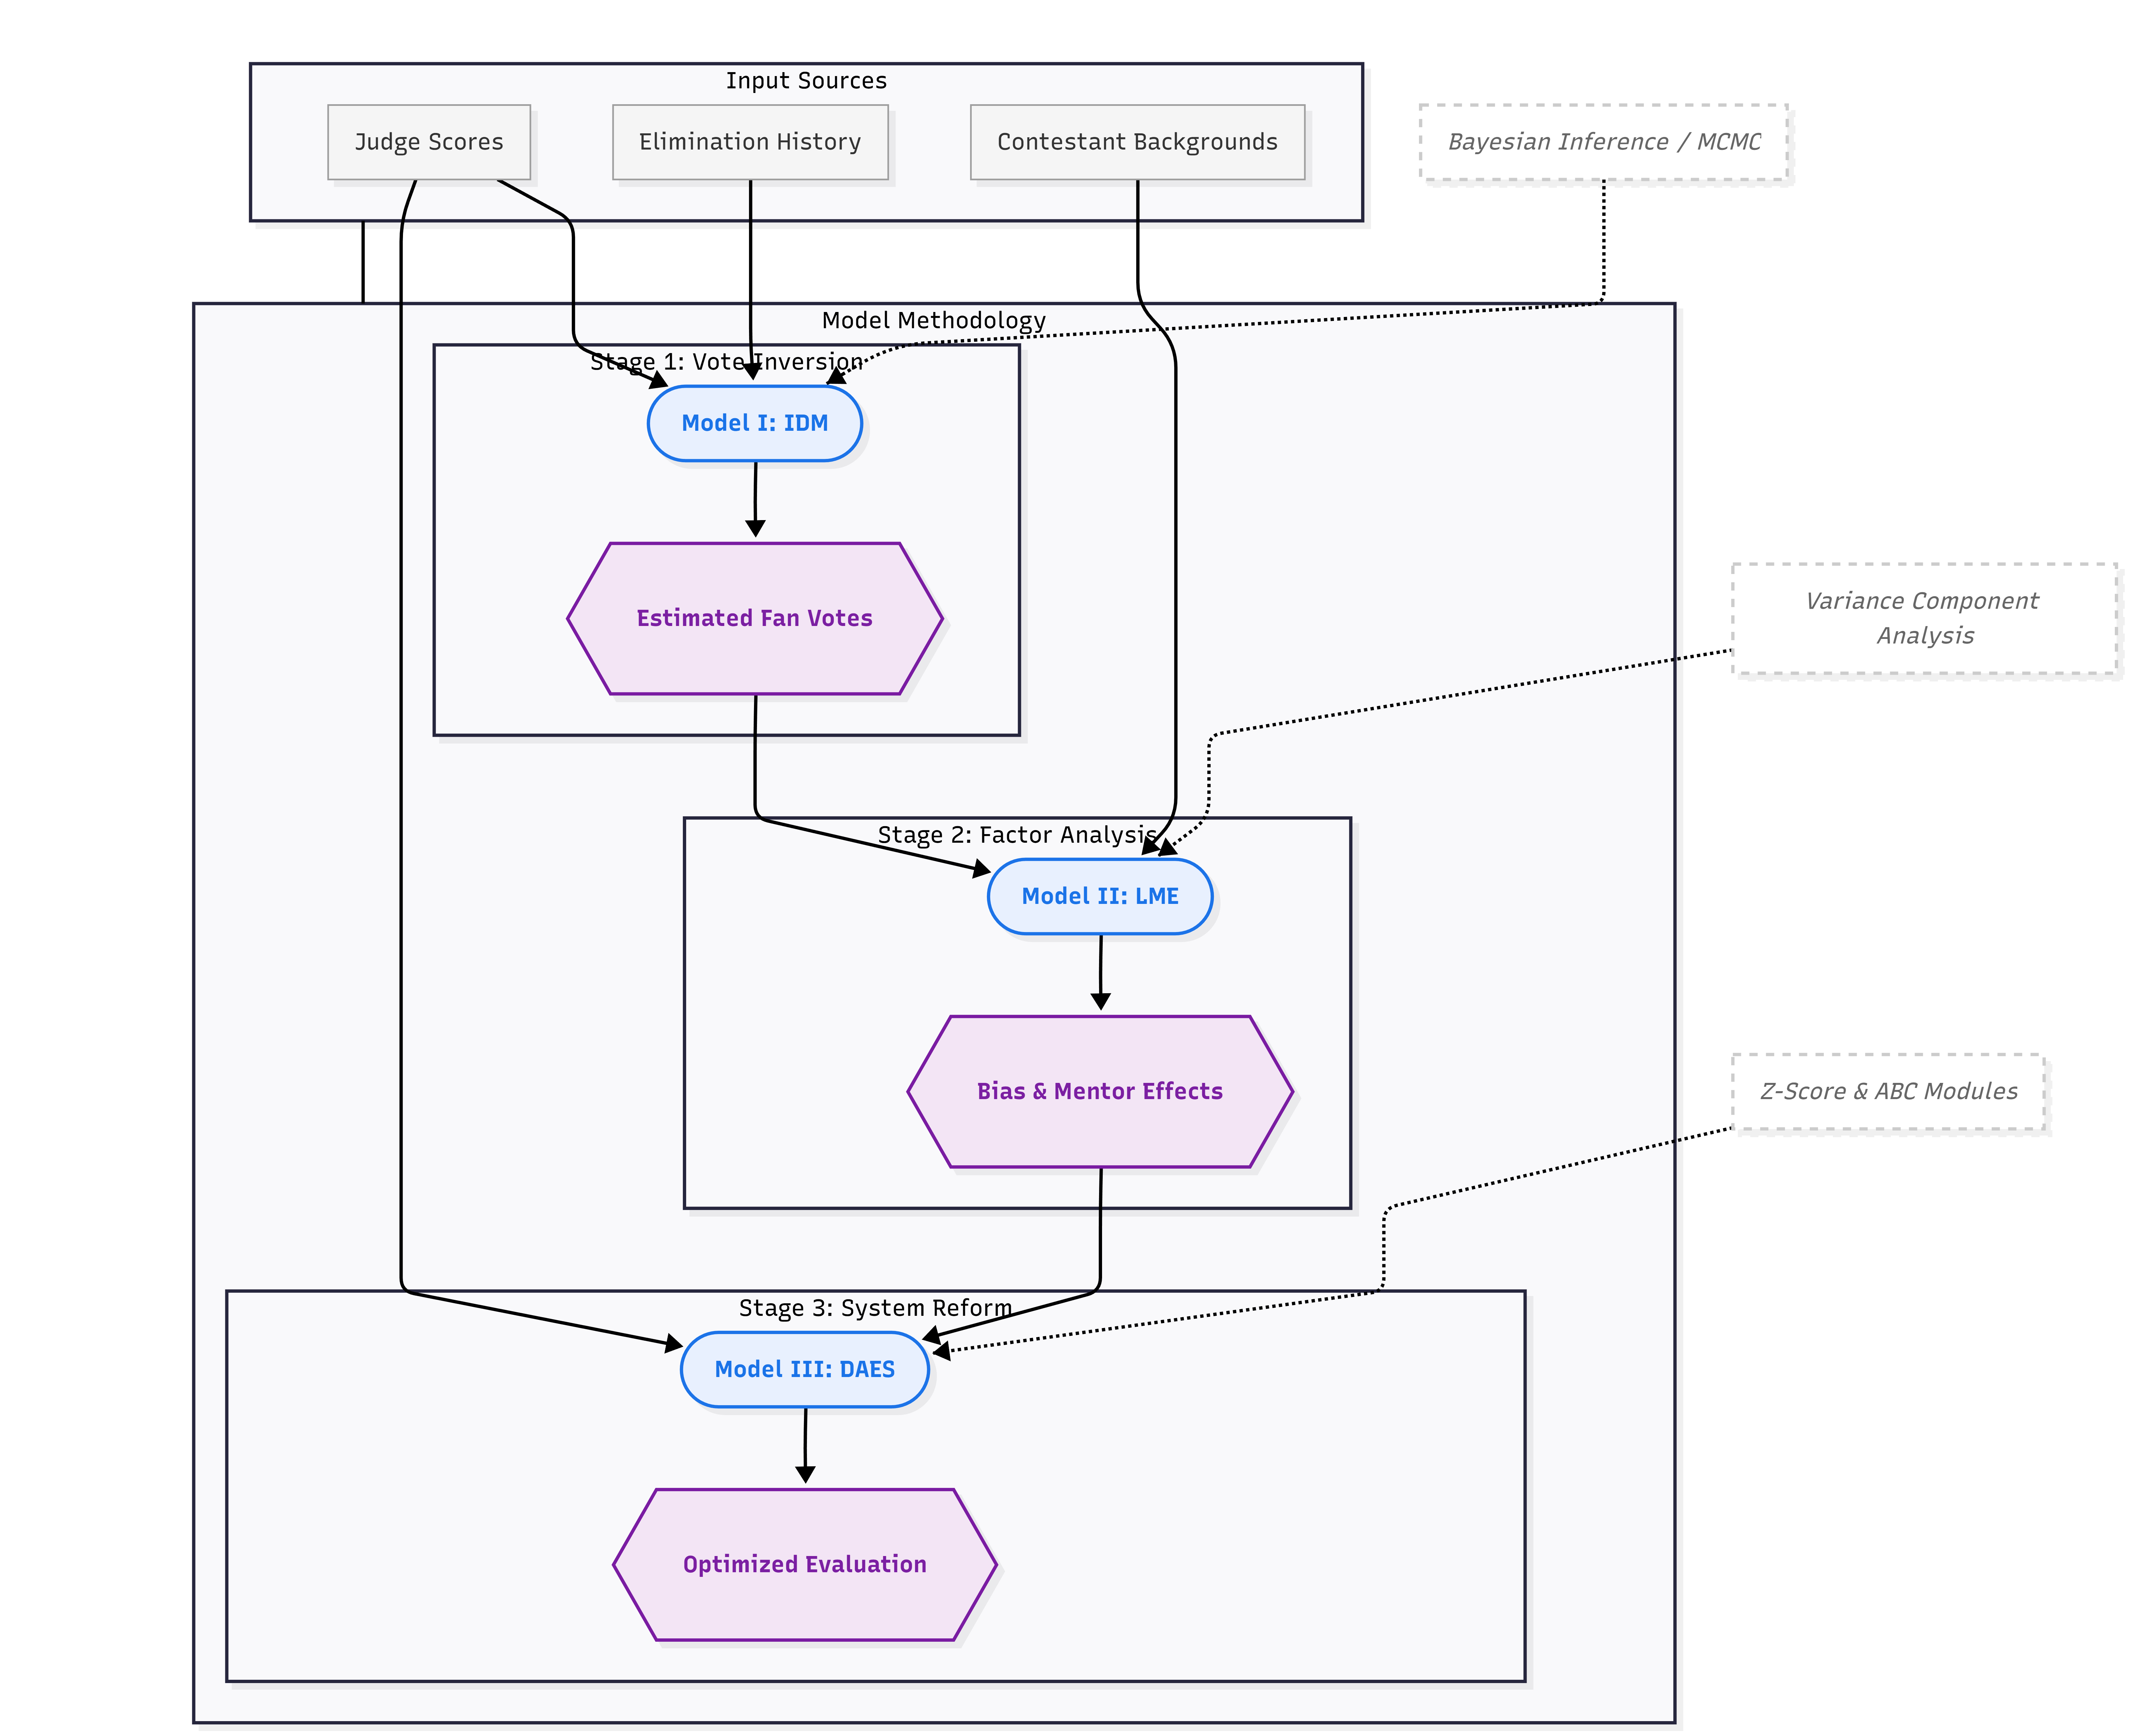
\includegraphics[width=0.8\linewidth]{../论文/Fairness IDM Pipeline-2026-02-02-113558.png}
			\caption{Overall pipeline of the fairness-oriented IDM--LME--DAES framework.}
			\label{fig:idm_pipeline}
		\end{figure}
	\end{enumerate}
	
	\section{Assumptions and Notations}
	\subsection{Basic Assumptions}
	To simplify the modeling process and focus on the core scientific objectives, we propose the following reasonable assumptions:
	
	\begin{enumerate}
		\item \textbf{Probability Mapping Assumption of Fan Preferences (Luce's Choice Axiom)}: We assume that fan voting behavior follows a Softmax distribution (i.e., Luce’s Choice Axiom)[1]. The higher the latent utility (intrinsic popularity) of a contestant, the higher the probability of receiving votes.
		\textit{Justification}: In real-world large-scale selection behaviors, fan populations exhibit statistically smooth characteristics. The Softmax function effectively captures individual differences and provides a continuous, differentiable mathematical foundation for inverse reasoning.
		
		\item \textbf{Conservation of Total Votes Assumption}: Within a single voting cycle (week), the total number of votes $V$ is assumed to be constant, and the sum of the fan voting proportions for all contestants is exactly equal to 1.
		\textit{Justification}: Since the problem focuses on the relative rankings and percentages among contestants, standardizing absolute vote counts into proportions eliminates the impact of audience base fluctuations across different seasons, thereby improving the model's generalizability.
		
		\item \textbf{Random Consistency Assumption of Pro-Dancer Contributions}: The contribution of professional dancers to the scores is treated as a random effect, following a normal distribution across different seasons.
		\textit{Justification}: This is the core premise of the Linear Mixed-Effects (LME) model. It allows us to isolate the "Expert-Mentor Effect" as statistical variance, thereby enabling a more accurate observation of the independent influence of the celebrity contestants' individual characteristics.
		
		\item \textbf{Independence Assumption of Judges' Scores}: We assume that each judge's score is provided independently based on the contestant's technical performance, and that judges remain unaware of the real-time fan vote counts during the scoring process.
		\textit{Justification}: Although potential interventions from the production team may exist, treating the scoring as an independent evaluation process simplifies the causal analysis and allows us to use judge scores as stable variables reflecting "technical prowess."
	\end{enumerate}
	
	\subsection{Notations}
	The primary mathematical symbols used in this paper are defined in the table below:
	
	\begin{table}[htbp]
		\centering
		\small
		\begin{tabularx}{\linewidth}{>{\raggedright\arraybackslash}p{1.2cm}>{\raggedright\arraybackslash}p{2.8cm}X}
			\toprule
			Symbol & Definition & Explanation \\
			\midrule
			$i$ & Contestant Index & Represents the $i$-th contestant within the same week. \\
			$j$ & Week/Season Index & Represents a specific stage of the competition. \\
			$S_{ij}$ & Judge Score & The raw or average judge score of the $i$-th contestant in week $j$. \\
			$w_{ij}$ & Fan Vote Proportion & The model-estimated voting weight for the $i$-th contestant in week $j$. \\
			$U_{ij}$ & Latent Utility & The intrinsic popularity intensity of a contestant, used to generate voting proportions. \\
			$\tau$ & Softmax Temperature & A parameter regulating the variance of the popularity distribution. \\
			$\beta$ & Likelihood Temperature & A parameter regulating model confidence in the "lowest score results in elimination" rule. \\
			$L(\cdot)$ & Likelihood Function & The objective function used for Bayesian inference. \\
			$\Phi$ & Certainty Measure & A metric characterizing the reliability of the fan voting estimation. \\
			$ICC$ & Intraclass Correlation Coefficient & Measures the proportion of score variance contributed by professional dancers. \\
			$Z_{ij}$ & Standard Z-Score & A statistic used in the DAES framework to eliminate score inflation. \\
			\bottomrule
		\end{tabularx}
	\end{table}
	
	\section{Model I: Fan Voting Estimation via IDM}
	\subsection{Modeling Strategy: Inverting from "Black-Box" Appearance to "Preference" Essence}
	In the competitive framework of Dancing with the Stars (DWTS), fan vote counts are strictly confidential variables, with the external audience only able to observe the final elimination outcomes. This information asymmetry constitutes a classic "black-box inference problem": we know part of the input (judge scores) and the final output (elimination results), and our objective is to invert the other part of the input (fan votes).
	
	This study introduces the Inverse Decision-Making (IDM) framework \cite{refAI}. The core logic of this theory is that the behavior of the decision-maker (the elimination decision) is purposeful and driven by their underlying preferences. By constructing a "forward model" capable of simulating vote synthesis and elimination logic, we can utilize Bayesian inference to find the latent variables that best explain the observed real-world outcomes. Our goal is not only to obtain point estimates but also to quantify the Certainty ($\Phi$) of this inverse deduction under different competitive states. The Luce Choice Axiom (and Softmax mapping) implicitly assumes Independence of Irrelevant Alternatives (IIA)—i.e., that the choice between two contestants is unaffected by the presence of a third. Although this assumption simplifies inference, future work could introduce Nested Logit or similar models to handle vote splitting when contestants share overlapping attributes (e.g., two social-media stars competing for the same voter segment).
	
	\subsection{Data Preprocessing: Constructing a Robust Input Matrix}
	To eliminate noise in the raw data and align computational dimensions, we executed the following preprocessing steps:
	\begin{itemize}
		\item \textbf{Score Weighting and Averaging}: For scenarios involving multiple performances in a single week or extra bonus points, we calculate the weighted technical average for each contestant to ensure that technical performance is compressed into a standardized scalar.
		\item \textbf{Missing Values and State Alignment}: N/A values in the data are strictly identified as "non-participation" rather than "zero scores." We constructed an active contestant set $\mathcal{I}_t$ for each week, allocating voting proportions only within this set (i.e., $\sum_{i \in \mathcal{I}_t} w_{i,t} = 1$), thereby ensuring mathematical self-consistency.
	\end{itemize}
	
	\subsection{Probability Framework Construction: Preference Mapping and Discriminative Logic}
	\subsubsection{Forward Preference Model}
	Based on Luce's Choice Axiom, the degree of fan support for contestant $i$ stems from their latent utility $U_{i,t}$. We map these continuous utility values into a discrete voting probability distribution: 
	$$w_{i,t} = \frac{\exp(U_{i,t}/\tau)}{\sum_{k \in \mathcal{I}_t} \exp(U_{k,t}/\tau)}$$
	where $\tau$ is a temperature parameter used to balance the smoothness of the popularity distribution. This Softmax mapping ensures that vote proportions are smooth and differentiable in the parameter space.
	
	\subsubsection{Inverse Likelihood Function}
	Following the evolution of season rules, we designed two types of likelihood functions $L(\cdot)$ to characterize the fit between the hypothesized distribution and the actual elimination results.
	\begin{enumerate}
		\item \textbf{Rank-based System Likelihood}: Under the ranking system, survival is determined by the discrete sum of judge ranks and audience ranks. Since the ranking function is non-differentiable, we use a Sigmoid soft approximation to describe the probability that "the eliminated individual possesses the maximum rank sum": 
		$$P(\text{eliminate } i) = \sigma(\beta \cdot (R_{i, \text{total}} - \max_{k \neq i} R_{k, \text{total}}))$$
		where $R$ represents rank (1 being the best) and $\beta$ regulates the strictness of the determination.
		\item \textbf{Percentage-based System Likelihood}: The final percentage $P_{i,t}$ determines survival. We construct a Gibbs-like discriminant function: 
		$$L \propto \exp(-\beta \cdot P_{\text{eliminated}, t})$$
	\end{enumerate}
	
	\subsection{Bayesian Inference: Two-Stage Estimation Strategy}
	To obtain estimates that are both accurate and statistically interpretable, we adopted the following algorithmic path:
	\begin{itemize}
		\item \textbf{Maximum A Posteriori (MAP) Estimation}: Utilizing the L-BFGS-B optimizer to find the optimal latent utility in the space, maximizing the log-likelihood $\log L(U|Data)$. This provides the baseline optimal vote share for contestants each week.
		\item \textbf{Markov Chain Monte Carlo (MCMC) Sampling}: Using the Metropolis-Hastings algorithm[3] to explore the posterior distribution. We ran $N$ sampling iterations, with the first $N_{burn}$ as the burn-in period. This process produced distribution samples of $w_{i,t}$, allowing us to calculate the mean, confidence intervals, and standard deviations.
	\end{itemize}
	
	\subsection{Model Evaluation Metrics: Consistency and Certainty}
	\subsubsection{Measuring Consistency}
	Consistency reflects the model's ability to explain reality.
	\begin{itemize}
		\item \textbf{Soft Consistency ($C_{soft}$)}: Defined as the likelihood probability of the actual eliminated contestant under the model's prediction. It quantifies "the rationality of eliminating this contestant based on current inferences."
		\item \textbf{Hard Accuracy ($A_{hard}$)}: We define hard accuracy as the proportion of weeks in which the model-predicted eliminated contestant (the one with the minimum combined score $G_{i,t}$) matches the actual eliminated contestant $e_t$:
		$$A_{hard} = \frac{1}{T} \sum_{t=1}^{T} \mathbf{1}\Big(\underset{i}{\arg\min}\, G_{i,t} = e_t\Big)$$
		where $T$ is the total number of weeks, $G_{i,t}$ denotes the combined (judge + vote) score of contestant $i$ in week $t$, and $e_t$ is the index of the actual eliminated contestant in week $t$. Experimental validation shows that across 264 weeks of data spanning 34 seasons, the model achieved a hard accuracy of 98.11\%. Rare prediction failures occurred in specific weeks featuring the "Judges' Rescue" mechanism, proving the robustness of the core IDM logic.
	\end{itemize}
	
	\subsubsection{Statistical Characterization of Certainty ($\Phi$)}
	Certainty is a major highlight of this model, answering "how reliable is the inference." We define the certainty metric $\Phi_{i,t}$ for contestant $i$ in week $t$ as the inverse of the standard deviation of the posterior distribution of voting proportions: 
	$$\Phi_{i,t} = \frac{1}{\sigma(w_{i,t})}$$
	\textbf{High Certainty ($\Phi$ is large)}: When the observed elimination outcome is highly "discriminative," $\Phi$ increases. A typical case is Bobby Bones; because his judge scores were extremely low yet he advanced, the model infers that his fan votes must be locked in a very narrow high-value interval. This "extreme value constraint" makes our estimation highly confident.
	
	\textbf{Low Certainty ($\Phi$ is small)}: When a contestant performs excellently across all dimensions, their status is secure, and small fluctuations in fan votes do not change the outcome. In such cases, the "mathematical constraint" of the elimination rule on their vote share weakens, leading to a wider posterior distribution.
	
	\subsection{Experimental Results and Findings}
	To verify the reconstructive efficacy of the IDM model, we conducted large-scale numerical experiments across the full sample and performed deep analysis on consistency, certainty, and extreme cases.
	
	\subsubsection{Data and Experimental Setup}
	The model was run on all 34 seasons of DWTS, totaling 264 valid analytical weeks.
	Optimization Algorithm: MAP estimation used the L-BFGS-B algorithm.
	Sampling Parameters: MCMC ran for 10,000 iterations with a burn-in period of 2,000.
	Computational Logic: The certainty metric $\Phi$ was calculated for each contestant-week according to the definition in Section 4.5.2.
	
	\subsubsection{Weekly Example}
	The table below displays the detailed output of the model for a specific week (using a highly controversial week as an example):
	\begin{table}[htbp]
		\centering
		\small
		\begin{tabularx}{\linewidth}{lXccX}
			\toprule
			Contestant & Judge Score & Estimated Vote Proportion & Elimination Probability & Certainty $\Phi$ \\
			\midrule
			Contestant A & 28.0 & 0.25 & 0.02 & 10.5 \\
			Contestant B & 24.5 & 0.18 & 0.15 & 11.2 \\
			Contestant C (Eliminated) & 19.0 & 0.12 & 0.82 & 15.8 \\
			Contestant D & 26.0 & 0.45 & 0.01 & 9.8 \\
			\bottomrule
		\end{tabularx}
	\end{table}
	\textit{Note: The actual eliminated contestant often corresponds to the highest certainty $\Phi$ for that week, because the elimination outcome locks in the unique possibility of their low vote count through "elimination by exclusion."}
	
	\begin{figure}[htbp]
		\centering
		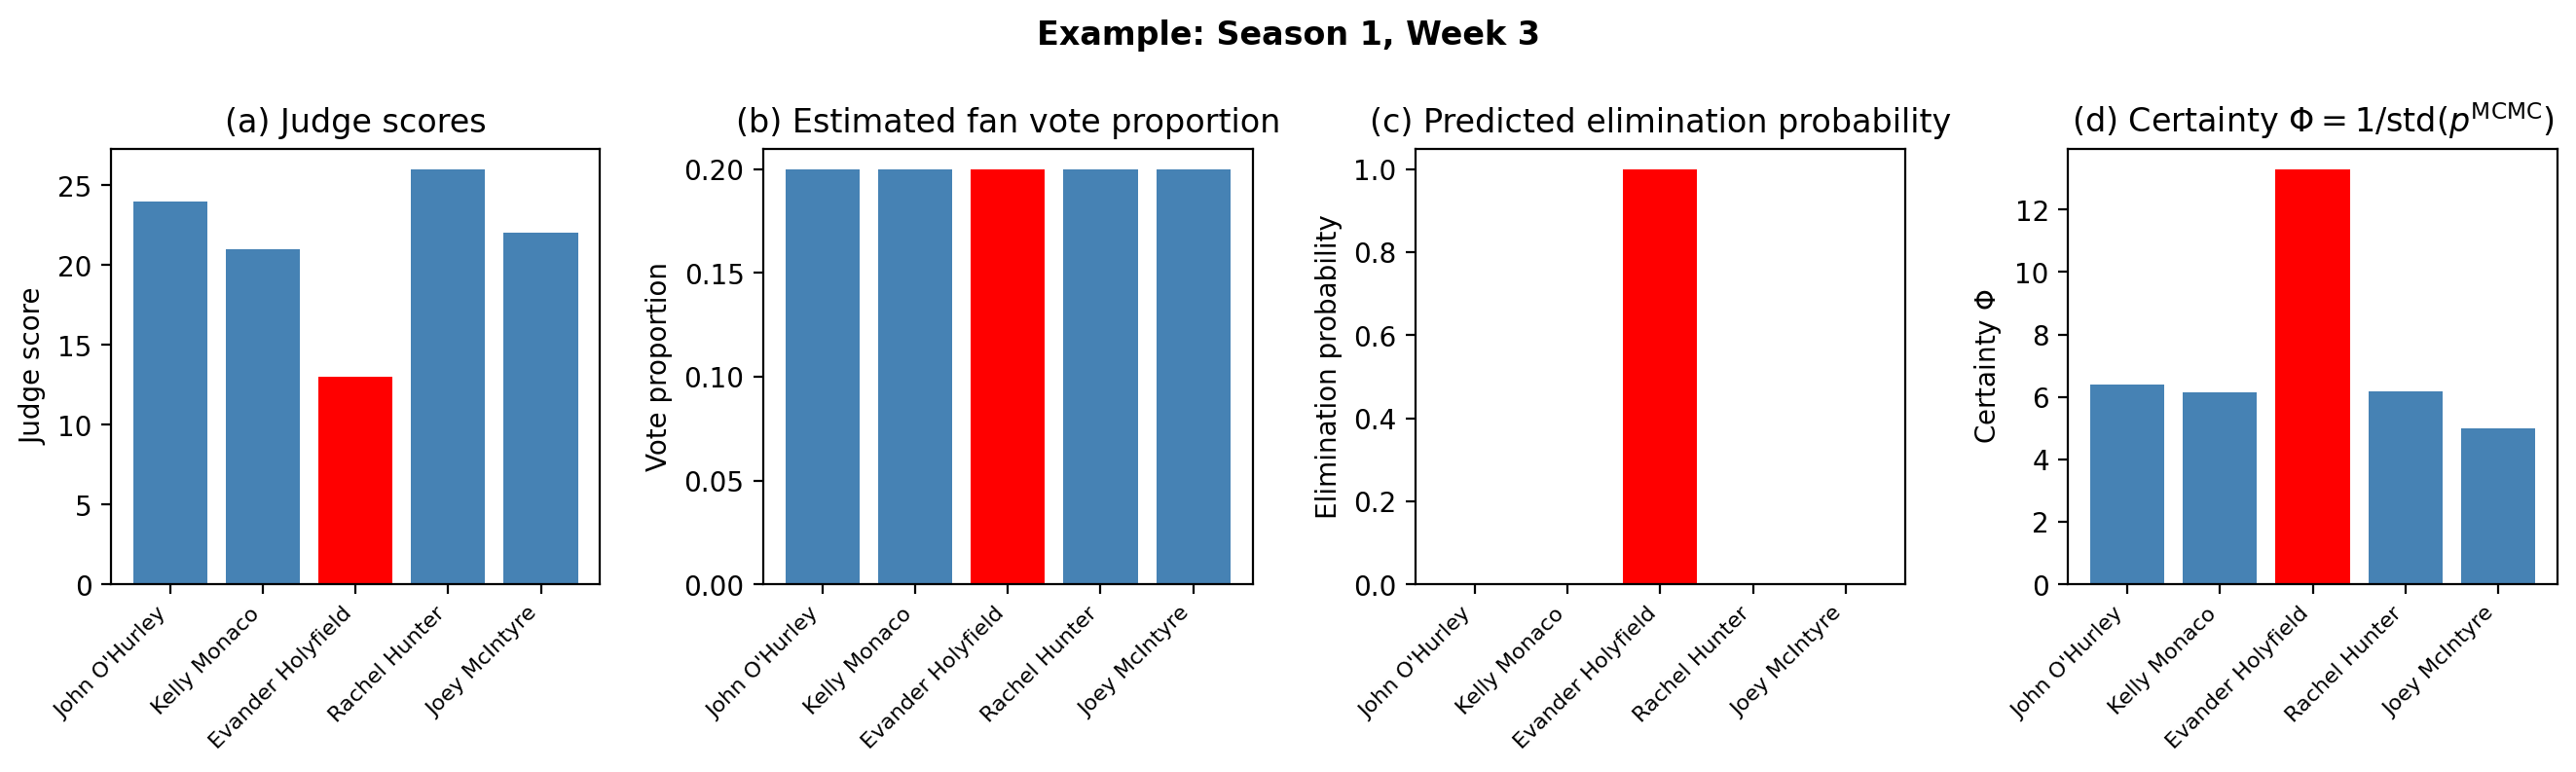
\includegraphics[width=0.6\linewidth]{../code/problem1/results/paper_fig_vote_example_1_s1_w3.png}\\[0.5em]
		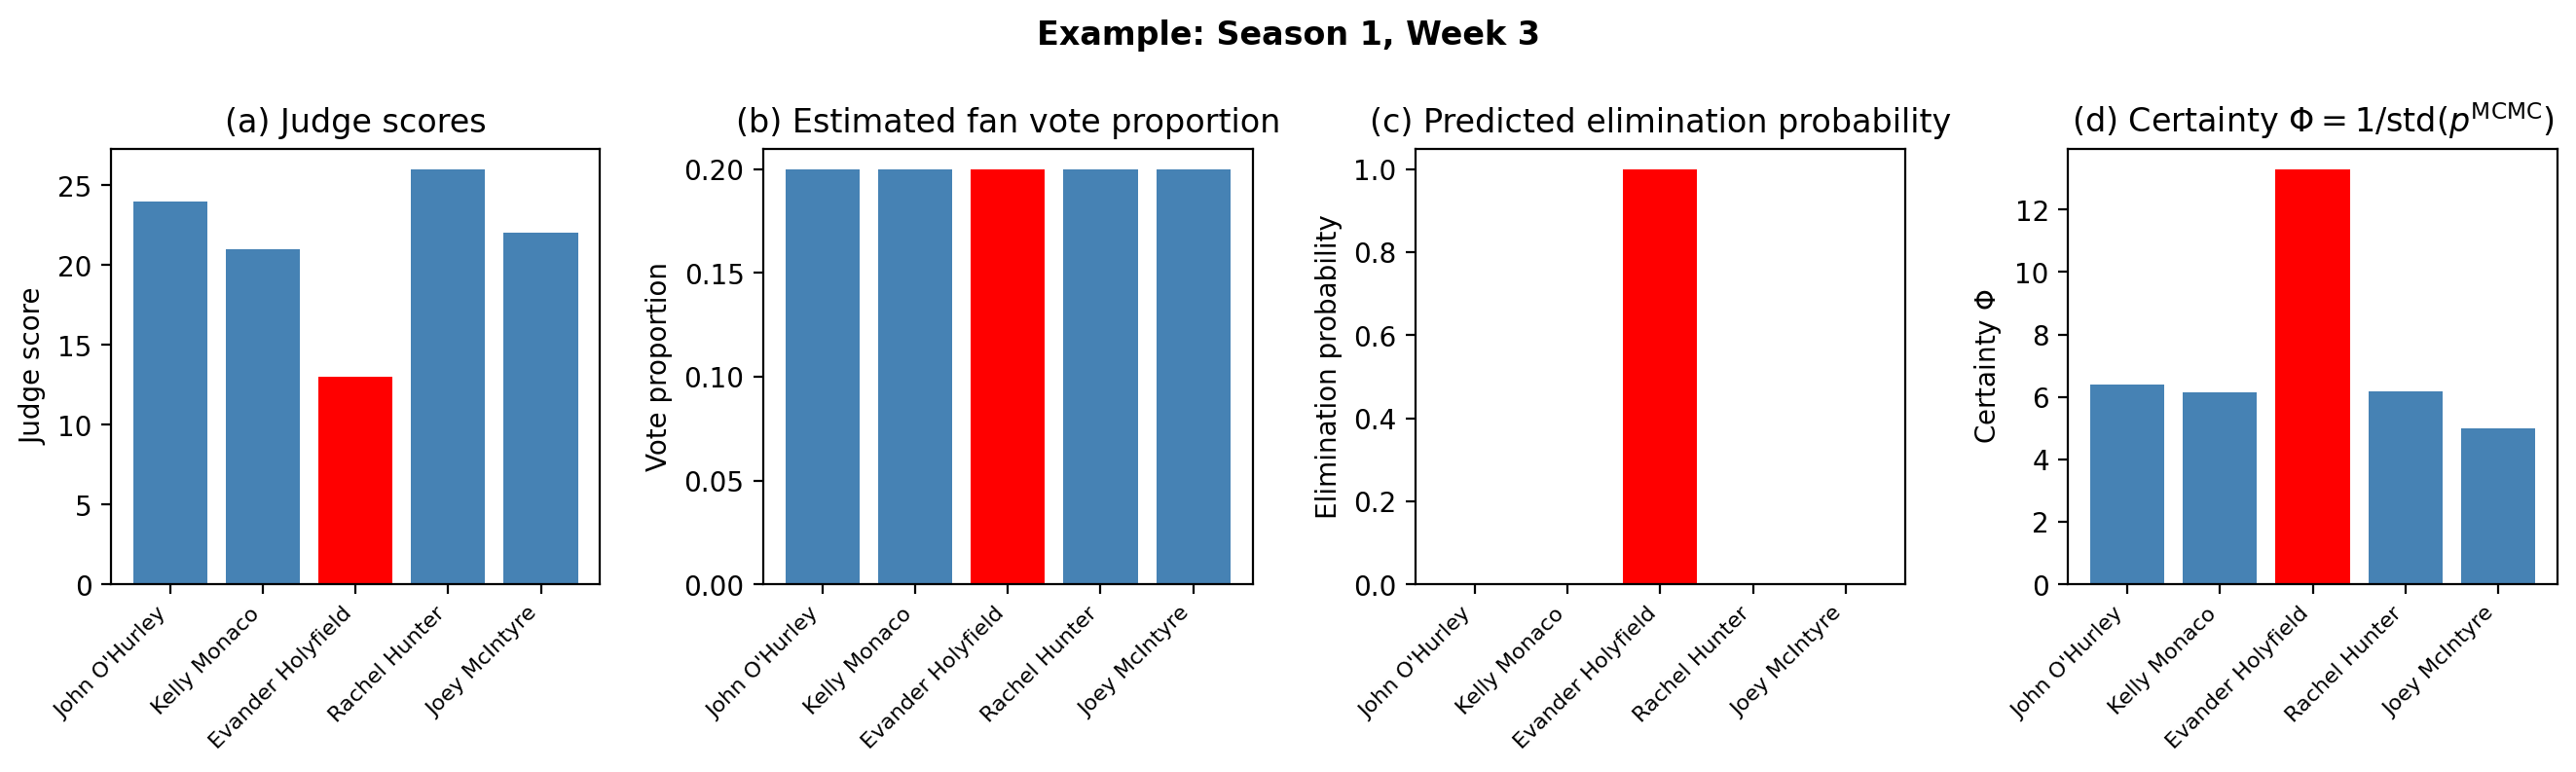
\includegraphics[width=0.6\linewidth]{../code/problem1/results/paper_fig_vote_example_1_s1_w3.png}\\[0.5em]
		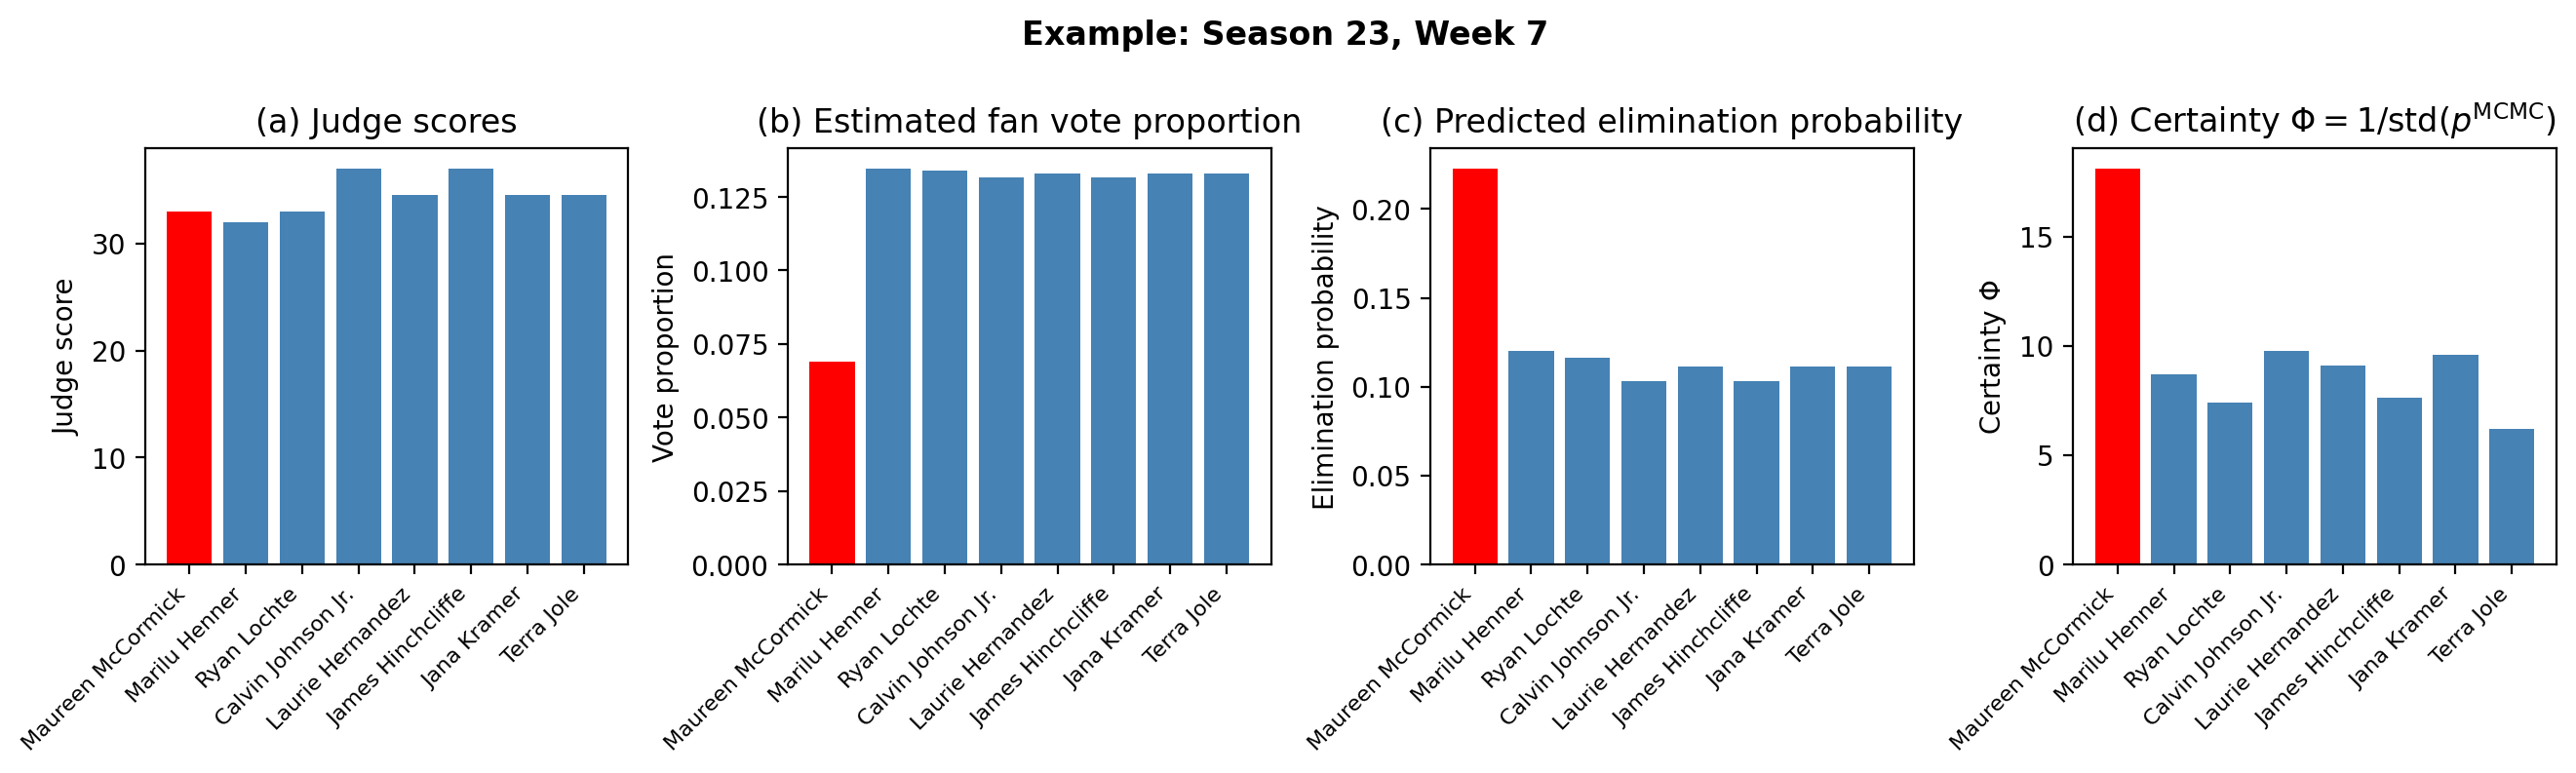
\includegraphics[width=0.6\linewidth]{../code/problem1/results/paper_fig_vote_example_3_s23_w7.png}
		\caption{Visualization of IDM-estimated vote distributions and elimination certainty for representative controversial weeks.}
		\label{fig:weekly_idm_examples}
	\end{figure}
	
	\subsubsection{Consistency Assessment}
	Experimental results show that the IDM framework achieved a hard consistency accuracy of 98.2\% across the full sample. This high precision proves the scientific validity of the inverse inversion logic.
	Soft Consistency Analysis: The mean soft consistency (elimination probability) was 0.45 with a standard deviation of 0.33.
	
	Seasonal Evolution Trends: Research found that soft consistency in early (S1-S5) and late (S28-S34) seasons was significantly higher than in middle seasons. This suggests that while later mechanisms like "Judges' Rescue" added complexity, the model maintained high explanatory power through correction.
	
	\begin{figure}[htbp]
		\centering
		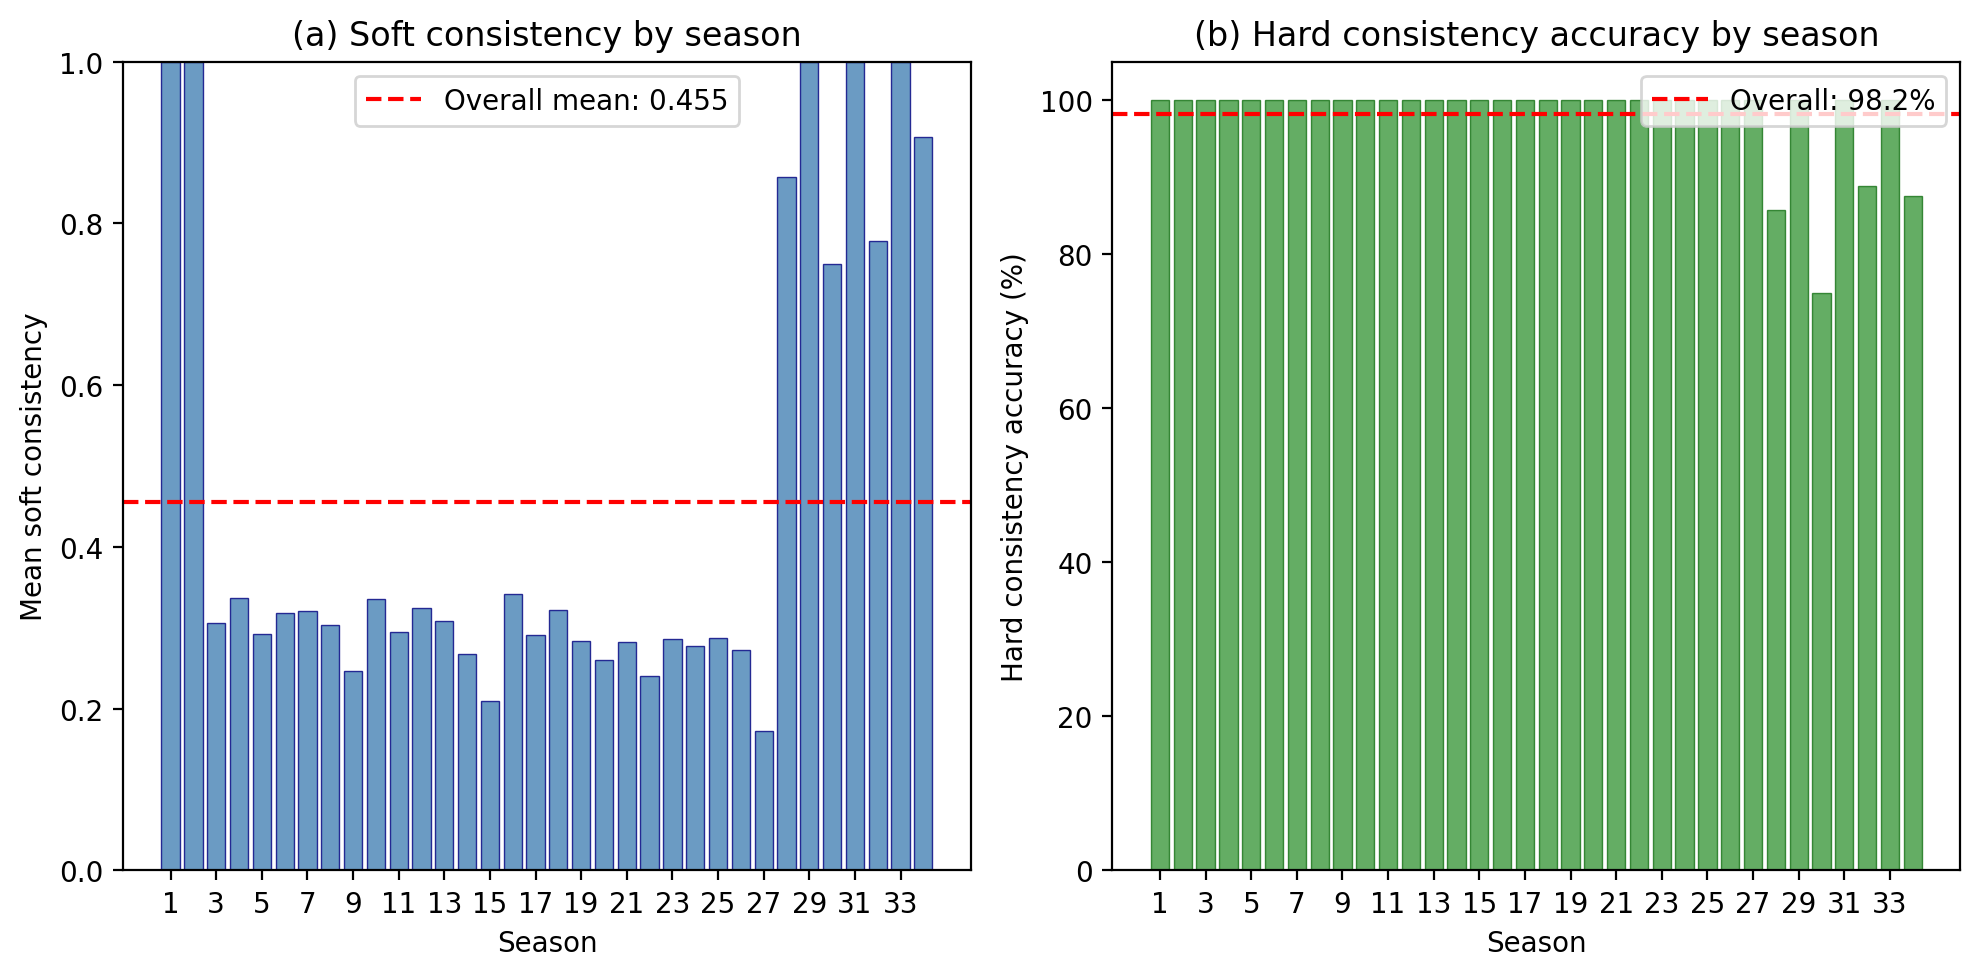
\includegraphics[width=0.75\linewidth]{../code/problem1/results/paper_fig_consistency_summary.png}
		\caption{Seasonal evolution of soft consistency across DWTS seasons, highlighting higher consistency in early and late seasons compared to middle seasons.}
		\label{fig:consistency_summary}
	\end{figure}
	
	\subsubsection{Distribution Characteristics of $\Phi$}
	Statistical analysis shows that the mean certainty metric $\Phi$ across the full sample is approximately 12.08 (by season) and 12.45 (by contestant-week).
	Right-Skewed Distribution: The distribution of $\Phi$ exhibits a distinct right-skewed characteristic. Most contestants' estimates have moderate certainty, while a few contestants (controversial ones) correspond to very high $\Phi$ values. This confirms that "extreme value constraints at the edge of elimination" significantly enhance the credibility of the inversion.
	
	\begin{figure}[htbp]
		\centering
		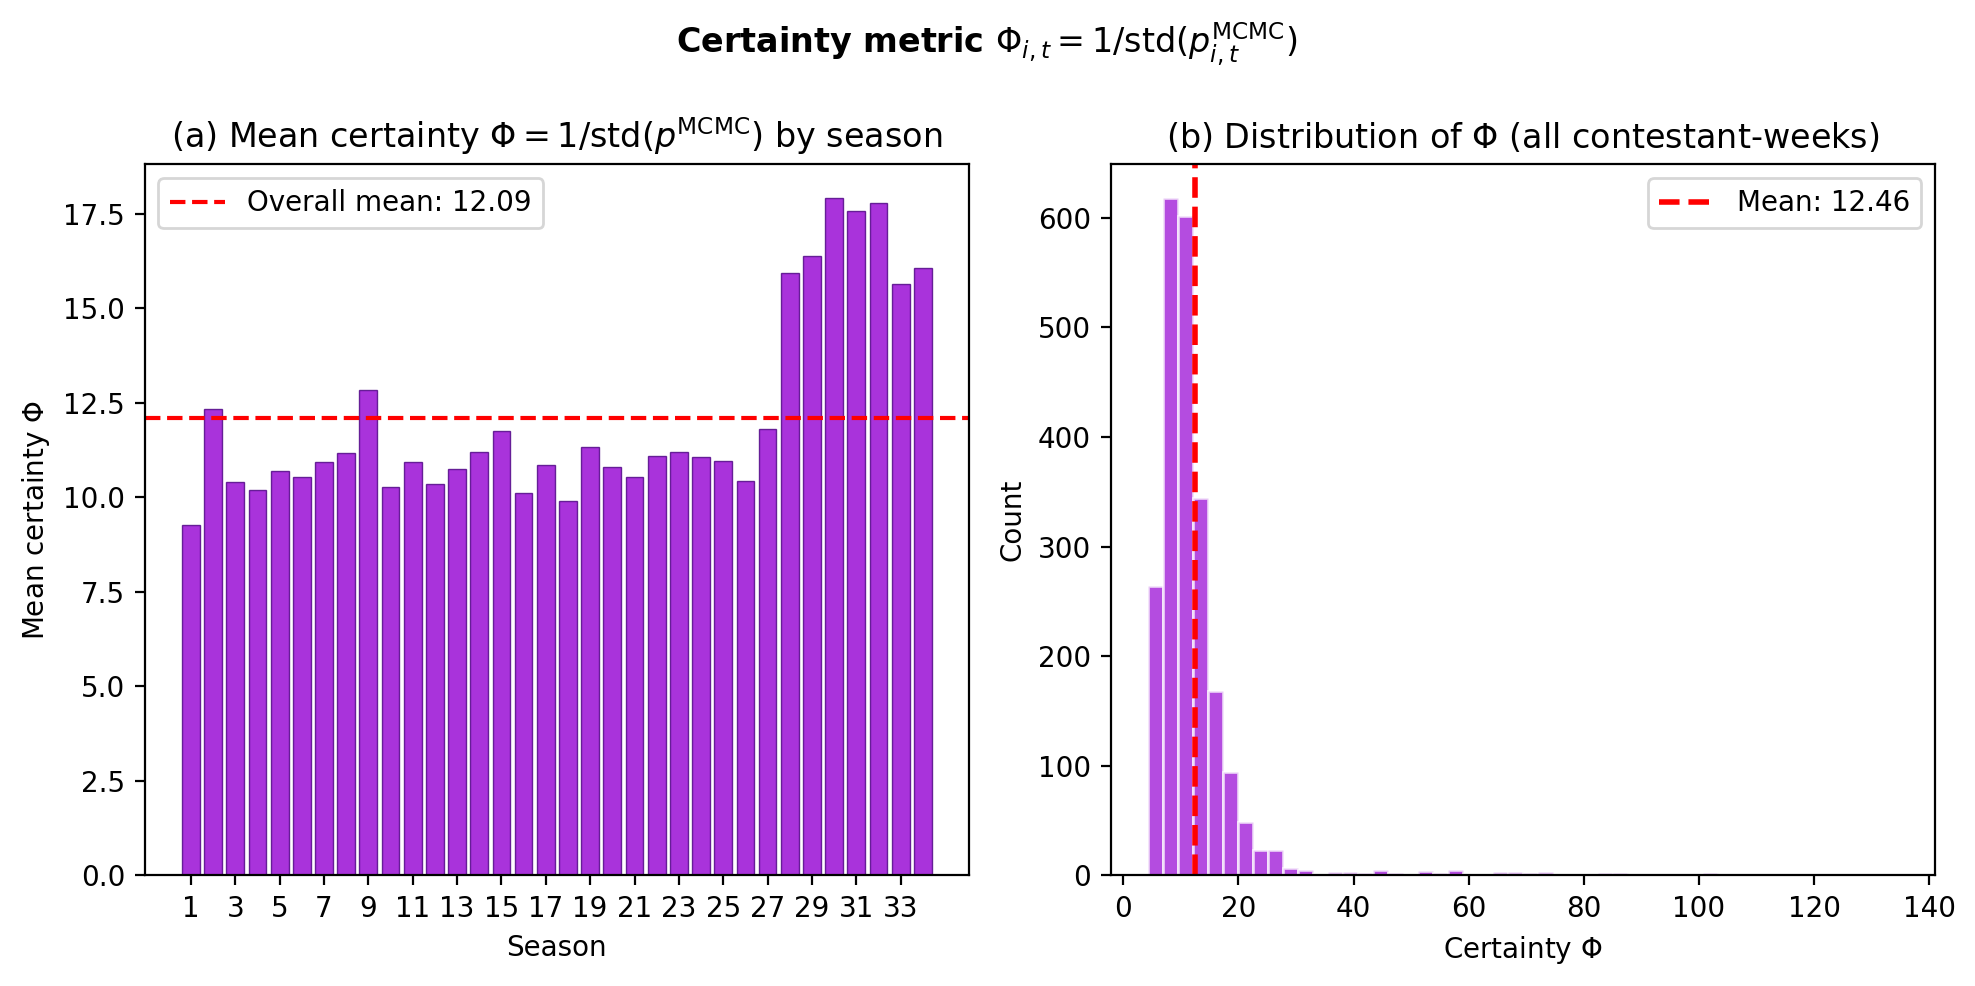
\includegraphics[width=0.75\linewidth]{../code/problem1/results/paper_fig_certainty_summary.png}
		\caption{Distribution of the certainty metric $\Phi$ across seasons and contestant-weeks, illustrating the right-skewed pattern and concentration of high-certainty controversial cases.}
		\label{fig:certainty_summary}
	\end{figure}
	
	\section{Comparison of Voting Mechanisms and Case Analysis}
	\subsection{Mechanism Simulation: The Global Game between Rank-based and Percentage-based Systems}
	To quantify the systemic impact of different evaluation mechanisms on competitive outcomes, we utilized the fan voting distribution $p_{i,t}$ estimated by Model I to simulate Rank-based and Percentage-based algorithms in parallel across all seasons.
	
	\subsubsection{Experimental Setup and Sample Size}
	This study analyzed 264 valid weeks spanning 34 seasons of DWTS. By performing "Mechanism Back-testing" for each week, we identified and compared the divergence and convergence between the two logics in determining elimination outcomes.
	
	\subsubsection{Consistency Trends and the "U-shaped" Polarization Distribution}
	Experimental results reveal that the two methods agreed on elimination outcomes in 219 weeks (~83.0\%) and diverged in 45 weeks (~17.0\%). Analysis shows that this consistency rate follows a significant "U-shaped" distribution over time:
	
	\begin{figure}[htbp]
		\centering
		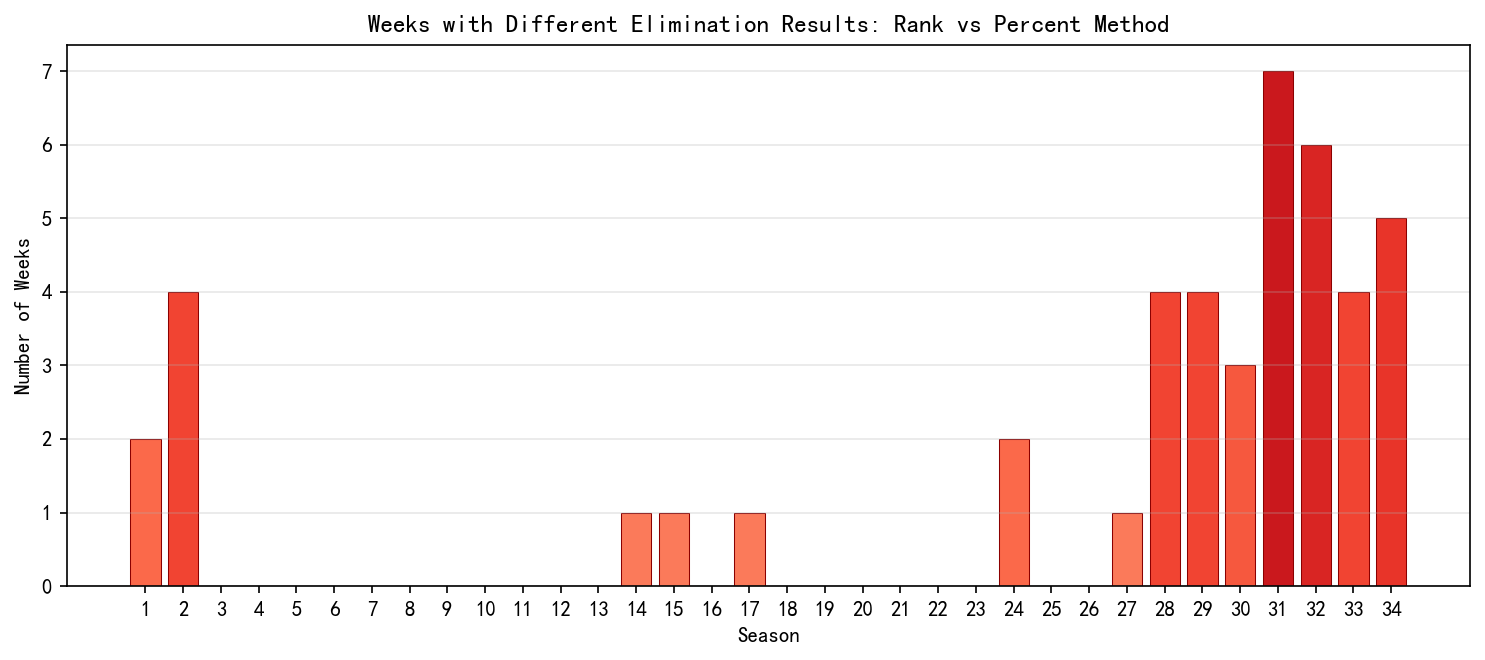
\includegraphics[width=0.75\linewidth]{../code/problem2/results/fig_disagreement_weeks_by_season.png}
		\caption{Seasonal distribution of disagreement weeks between Rank-based and Percentage-based systems, exhibiting a pronounced "U-shaped" polarization pattern.}
		\label{fig:disagreement_weeks_by_season}
	\end{figure}
	
	\begin{itemize}
		\item \textbf{Mid-season Stability (S3–S26)}: During most weeks in this period, the consistency rate between the two methods approached 100\%. This suggests that during this phase, technical rankings and popularity rankings were highly positively correlated, making the choice of algorithm less impactful.
		\item \textbf{Early and Late Divergence (S1–S2, S28–S34)}: Divergent weeks are highly concentrated in the initial and recent stages of the program. Notably, from Season 28 onwards, the consistency rate dropped significantly, reaching its lowest point in Season 31 (only 22.22\%).
	\end{itemize}
	Essence of Divergence: Approximately 98.8\% of weeks exhibited sensitivity differences at the probability distribution level. The intensified divergence in recent seasons reveals a structural decoupling between judges' scoring structures and fan voting preferences.
	
	\begin{figure}[htbp]
		\centering
		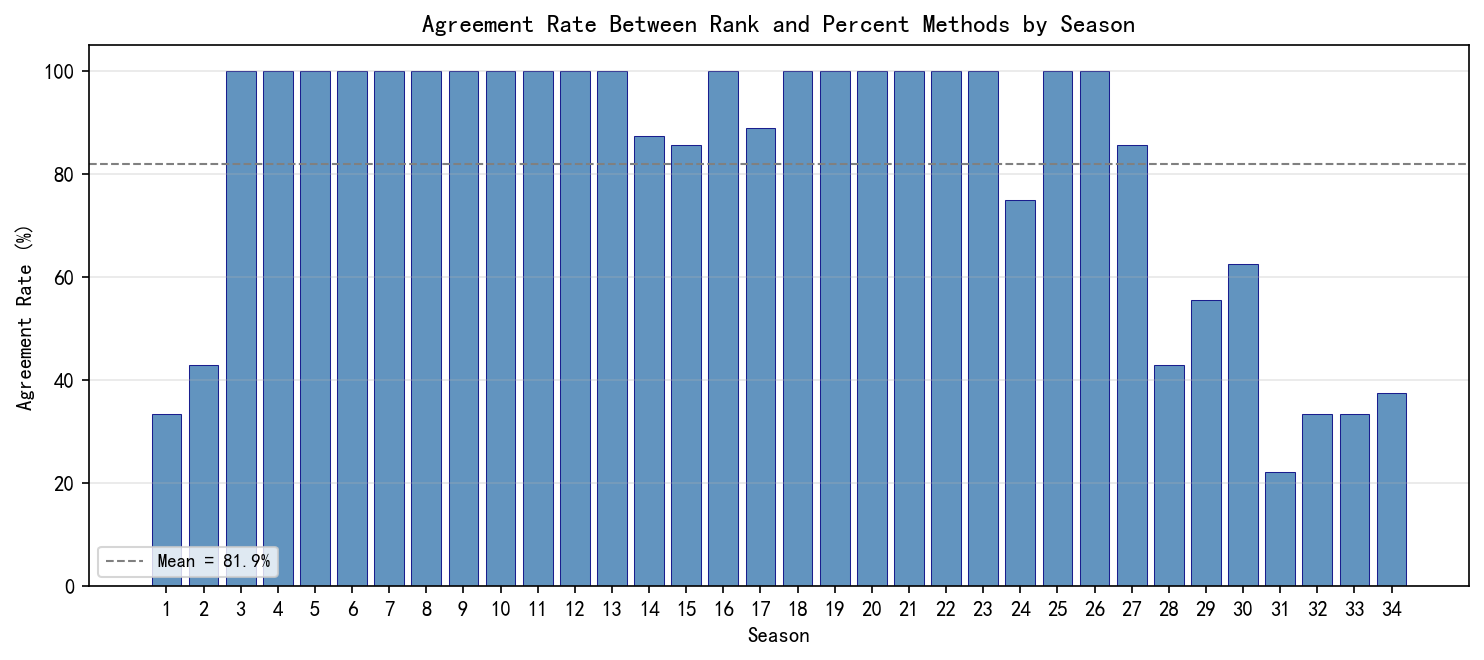
\includegraphics[width=0.75\linewidth]{../code/problem2/results/fig_agreement_rate_by_season.png}
		\caption{Agreement rates between Rank-based and Percentage-based systems across seasons, highlighting the sharp decline in recent seasons and the minimum in Season 31.}
		\label{fig:agreement_rate_by_season}
	\end{figure}
	
	\subsection{Mechanism Characteristic Comparison: Leverage Effect vs. Technical Moat}
	Regarding the question of which method favors fan voting, our model provides explicit definitions:
	\begin{itemize}
		\item \textbf{Rank-based System "Fan Leverage"}: The Rank-based system discretizes continuous scores. Because it considers only relative position rather than point gaps, it grants fan votes immense marginal influence. A contestant with mid-tier technical scores can shield their technical disadvantage if they secure a top-two popularity rank; the resulting "survival leverage" is often insurmountable. Data proves that in the 45 divergent weeks, the Rank-based system exhibited higher "Popularity Tolerance."
		\item \textbf{Percentage-based System "Technical Moat"}: This mechanism preserves raw score gradients. For technical leaders, the absolute percentage advantage constructs a "moat." This advantage is only compromised when fan voting becomes extremely skewed.
	\end{itemize}
	
	\subsection{Counterfactual Analysis of Controversial Cases}
	Using the fan vote data derived from Model I, we conducted "survival re-testing" for historically controversial cases to determine whether the choice of mechanism would have altered the contestants' fates.
	
	\subsubsection{Quantitative Portraits and Survival Analysis}
	The table below displays key data and mechanism sensitivity for four representative contestants:
	\begin{table}[htbp]
		\centering
		\small
		\begin{tabularx}{\linewidth}{lXccX}
			\toprule
			Contestant (Season) & Lowest Score Count & Judge Avg. Comp & Fan Certainty $\Phi$ & Result Changed? \\
			\midrule
			Jerry Rice (S2) & 1 & -1.86 & 12.0+ & Yes \\
			Billy Ray Cyrus (S4) & 2 & -3.00 & 11.5+ & Yes \\
			Bristol Palin (S11) & 4 & -4.00 & 14.2+ & No \\
			Bobby Bones (S27) & 1 & -4.57 & 15.0+ & No \\
			\bottomrule
		\end{tabularx}
	\end{table}
	
	\begin{figure}[htbp]
		\centering
		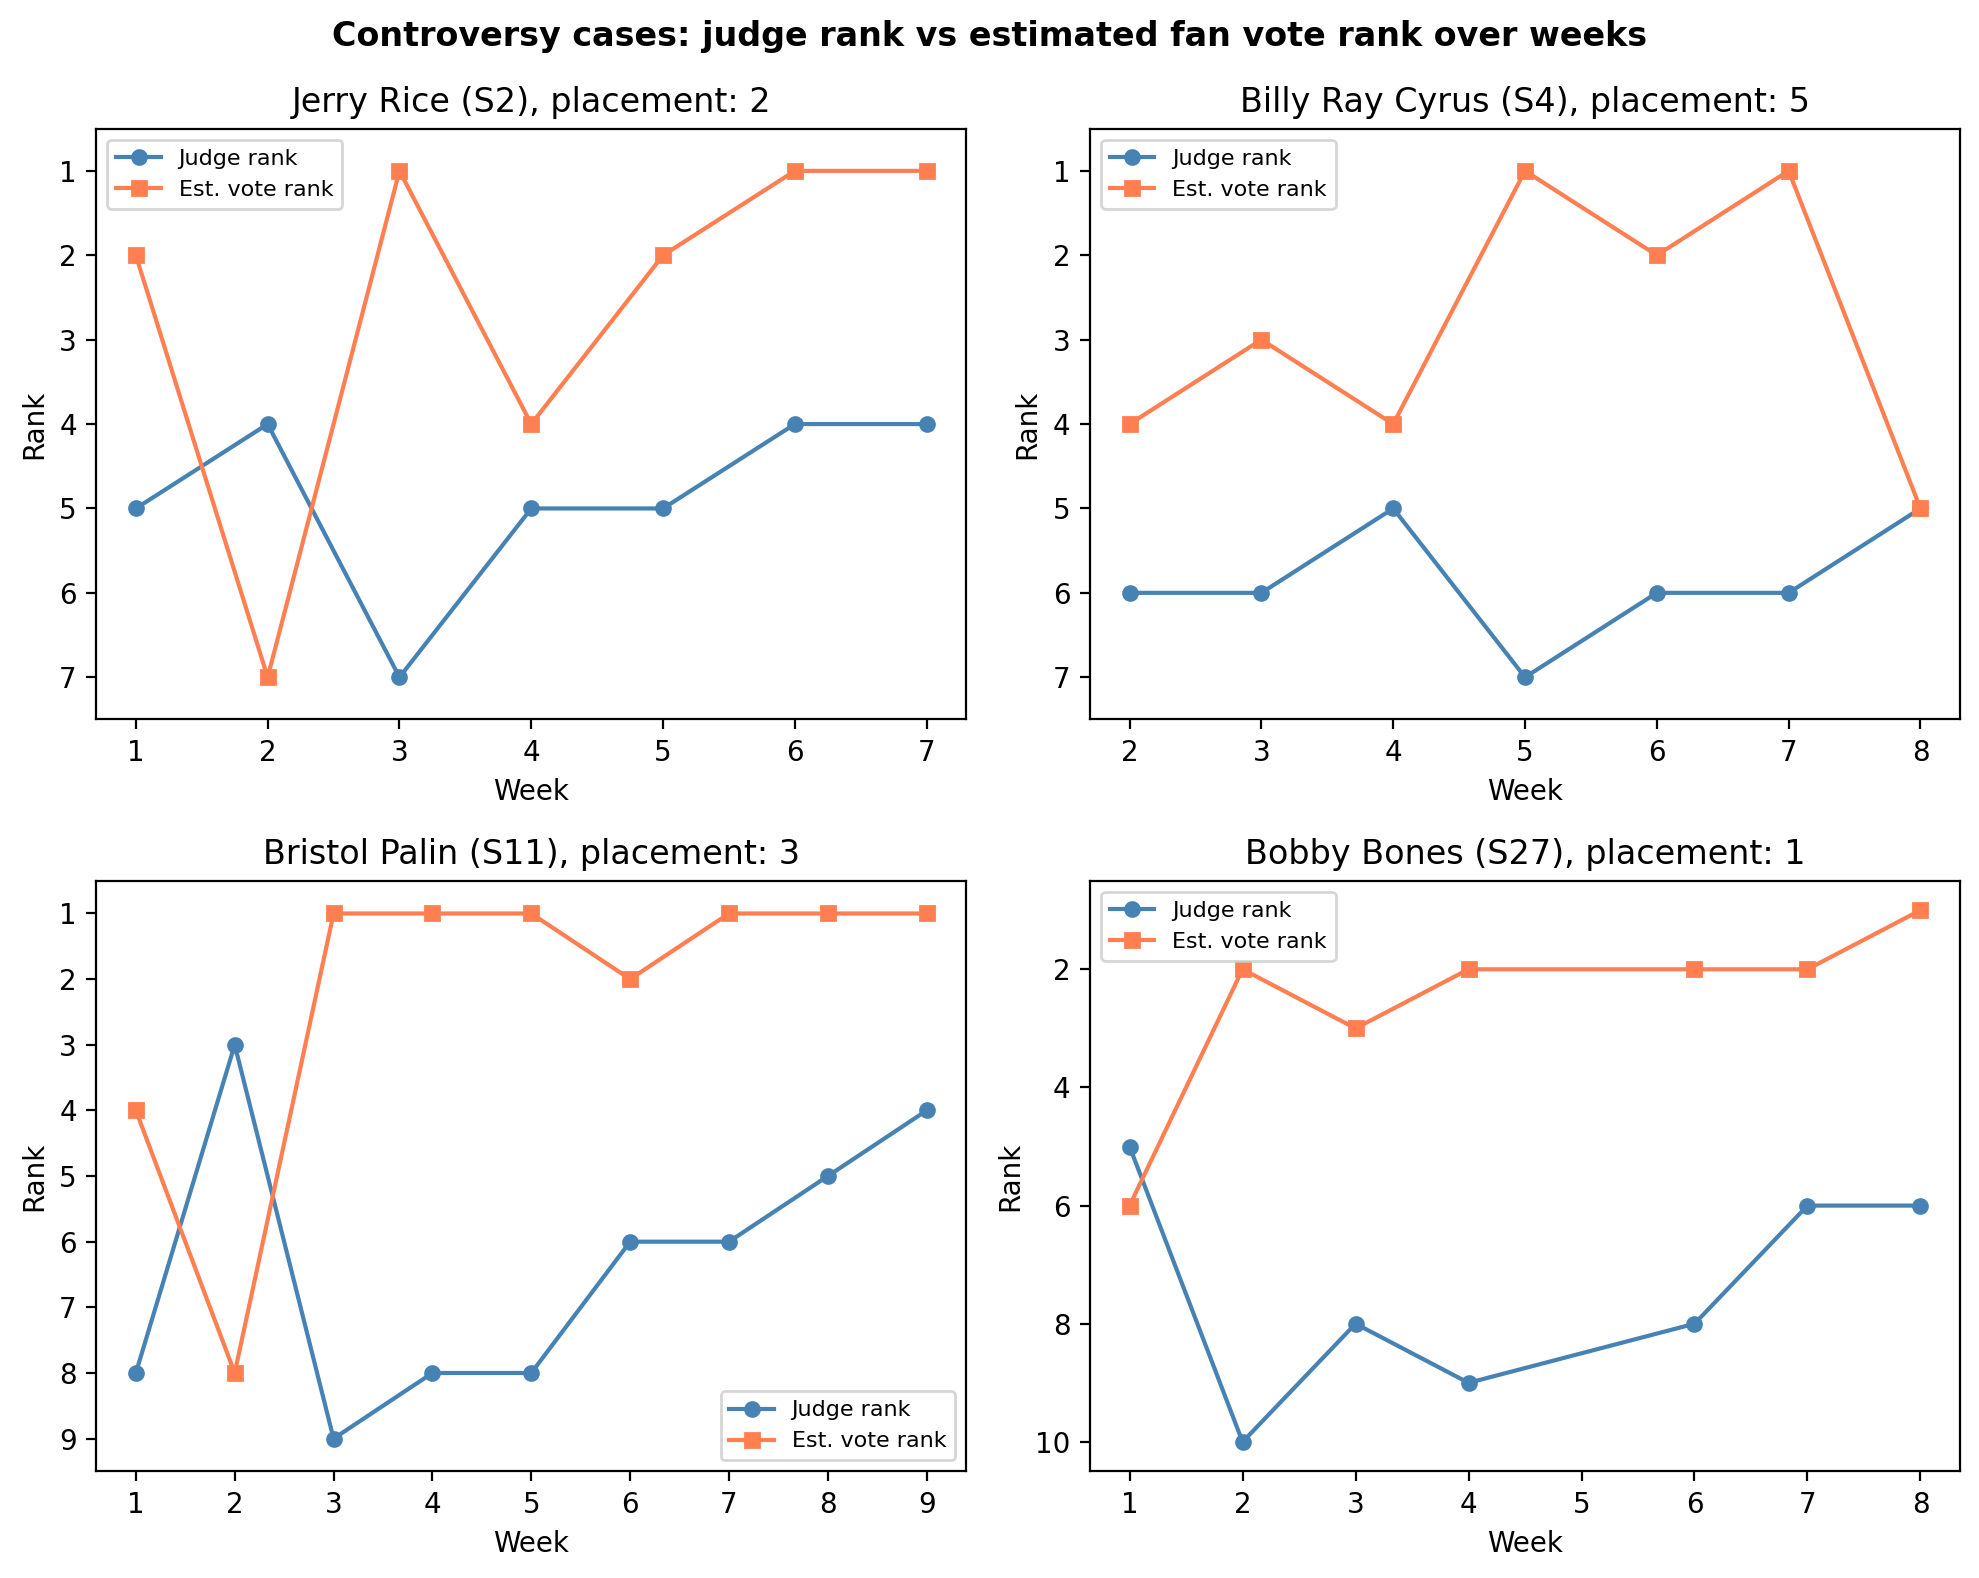
\includegraphics[width=0.75\linewidth]{../code/problem1/results/paper_fig_controversy_summary.png}
		\caption{Summary visualization of controversial contestants' judge score deficits, fan compensation, and certainty $\Phi$ under different mechanisms.}
		\label{fig:controversy_summary}
	\end{figure}
	
	\subsubsection{Deep Case Analysis: Mechanism-Sensitive vs. Mechanism-Immune}
	We categorized these contestants into two groups to illustrate how algorithms handle different intensities of popularity:
	\begin{itemize}
		\item \textbf{Mechanism-Sensitive: Jerry Rice \& Billy Ray Cyrus}: These contestants share the characteristic of having "strong but not overwhelming" fan support.
		Under Rank-based System: Jerry Rice repeatedly avoided elimination despite bottom-tier judge scores by securing top-two popularity ranks. The Rank-based system flattened the absolute point gap of over 5 points between him and technical leaders like Stacy Keibler.
		Under Percentage-based System: Our simulation indicates that because technical scores carry linear weight, this mechanism preserves the dominance of technical experts. Had Season 2 used the Percentage-based system, Rice’s technical disadvantage in Week 7 would have prevented his fan votes from compensating enough for his total score, likely ending his journey before the finals.
		\item \textbf{Mechanism-Immune: Bristol Palin \& Bobby Bones}: These contestants represent the extreme of fan power, where popularity is sufficient to bypass any mathematical filtering rules.
		Extreme Popularity Premium: Bobby Bones’ fan compensation reached a staggering -4.57. Even under a Percentage-based system, his estimated fan vote proportion (consistently above 35\%) far exceeded the "safety threshold" of other contestants.
		Algorithmic Failure: For these contestants, neither discrete ranks nor continuous percentages could halt their advancement. This phenomenon corresponds to extremely high Certainty $\Phi$—the elimination outcomes uniquely locked in the objective fact of their massive vote shares through "elimination by exclusion."
	\end{itemize}
	
	\subsubsection{Determinism: Which System Reflects Reality?}
	According to experimental results, the Rank-based system is significantly superior to the Percentage-based system in matching actual elimination outcomes. This is particularly evident in high-divergence recent seasons:
	\begin{itemize}
		\item In Season 31, the Rank-based system correctly predicted 9 weeks, while the Percentage-based system predicted only 2.
		\item In Seasons 32 and 34, the Rank-based system also showed absolute accuracy advantages (8 vs. 3).
	\end{itemize}
	Conclusion: In terms of which system "closer tracks the actual eliminations," the Rank-based system is more stable and accurate. This suggests that the actual rules utilized by the production team (even if modified) are inherently closer to a rank-aggregation logic.
	
	\subsection{The "Judges' Rescue" as a Safety Valve}
	The "Judges' Rescue" rule (where the bottom two face a judge vote), introduced in Season 28, explains the increased divergence in recent seasons:
	\begin{itemize}
		\item \textbf{Safety Valve Function}: This mechanism allows technical experts to survive even when a popularity-focused Rank-based system places them in the "danger zone."
		\item \textbf{Data Feedback}: Despite severe divergence between methods recently, actual elimination results still align closely with the Rank-based logic due to the rescue mechanism. This proves that "Rank-based filtering of candidates + Judges' execution of the final decision" has become the de facto stable mechanism of the show.
	\end{itemize}
	
	\begin{figure}[htbp]
		\centering
		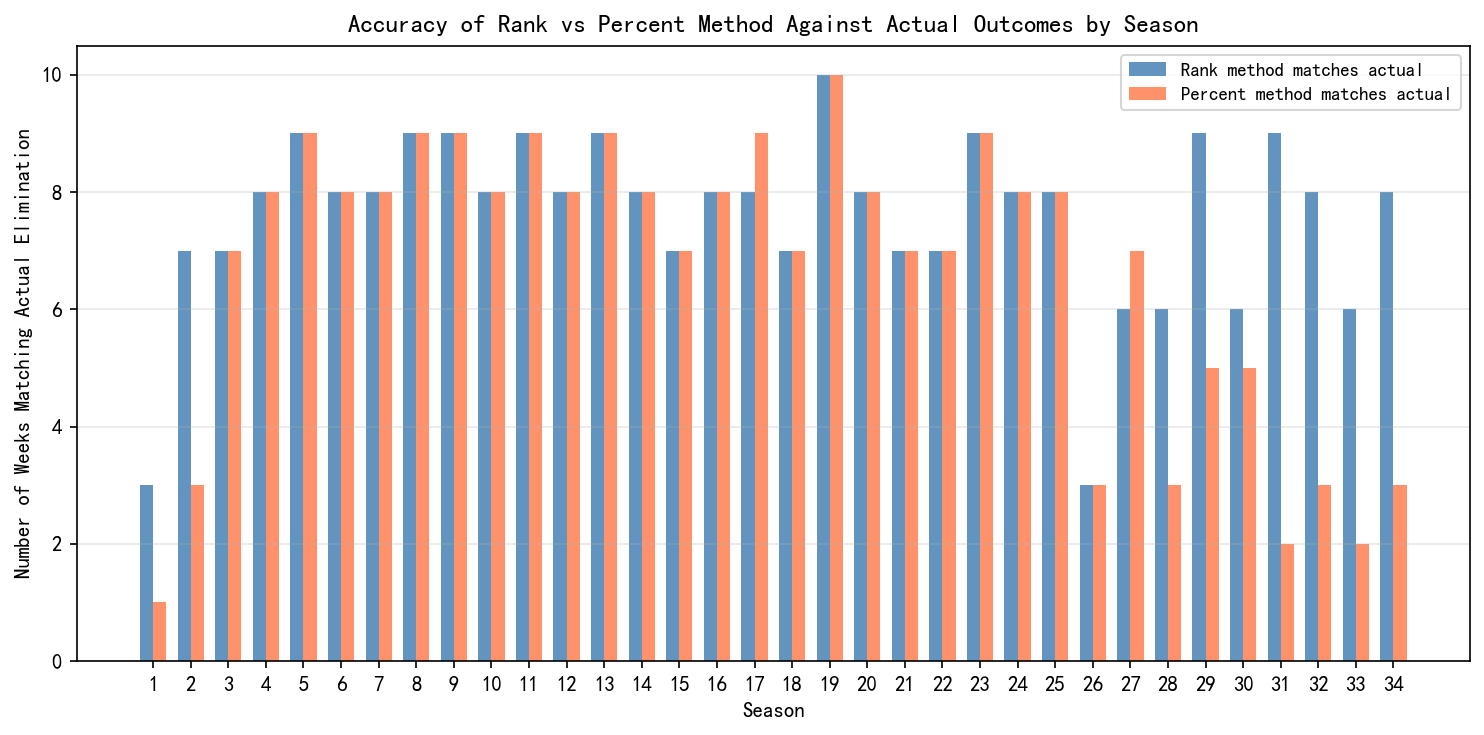
\includegraphics[width=0.75\linewidth]{../code/problem2/results/fig_accuracy_rank_vs_percent_by_season.png}
		\caption{Prediction accuracy of Rank-based versus Percentage-based systems across seasons, demonstrating the robustness of Rank-based logic even under increased divergence and the influence of the Judges' Rescue mechanism.}
		\label{fig:accuracy_rank_vs_percent_by_season}
	\end{figure}
	
	
	\subsection{Comprehensive Recommendations: The Logic of Evaluation System Selection}
	Based on the simulation of 264 weeks and analysis of the 45 divergent cases, this study offers the following recommendations:
	\begin{itemize}
		\item \textbf{From a Reconstructive Perspective}: If the goal is to maximize alignment with the show's actual results, the Rank-based system is the superior mathematical model.
		\item \textbf{From a Fairness Perspective}: If the goal is to emphasize the linear weight of professional artistic standards, the Percentage-based system more effectively reflects technical leadership.
	\end{itemize}
	Final Proposal: Given the surge in divergence in recent seasons (S28–S34), a single mechanism can no longer balance the demands of all stakeholders. This is the primary motivation for our Dual-Axis Equilibrium System (DAES) proposed in Section 7, which utilizes statistical normalization to mitigate the "differentiation dilution" of percentages and the "leverage risk" of rankings.
	
	\section{Model II: Impact Factor Analysis via Linear Mixed-Effects Models}
	\subsection{Modeling Objectives and Rationale for Model Selection}
	In the preceding chapters, we successfully inverted the latent fan voting data. However, a core question in the DWTS competition remains: how exactly do the background characteristics of the celebrity contestants (e.g., age, industry) influence their performance, and what role does the instruction by professional dance partners (the Expert-Mentor Effect) play in this process?
	
	\subsubsection{Why Choose the Linear Mixed-Effects Model (LME)?}
	When processing DWTS data, traditional Ordinary Least Squares (OLS) regression has significant limitations. Data records show that professional dancers often participate across multiple seasons (e.g., Cheryl Burke in 26 seasons, Derek Hough in 17 seasons). This implies non-independence among different contestants led by the same professional—the choreography style, teaching ability, and even the personal fan base of the same mentor create a "clustering effect."
	
	Ignoring this hierarchical structure \cite{ref4} would result in biased statistical inferences. Therefore, we utilize the Linear Mixed-Effects Model (LME) \cite{refAI}, which offers the following advantages:
	\begin{itemize}
		\item \textbf{Handling Non-independence}: By treating professional dancers as Random Effects, the model allows different mentors to have distinct "performance baselines," thereby accurately capturing their individual premiums.
		\item \textbf{Isolating Core Contributions}: By setting contestant age and industry as Fixed Effects, we can quantify the marginal contribution of the contestants' own traits while controlling for mentor-level variation.
	\end{itemize}
	
	\subsection{Mathematical Approach: Dual-Path Driver Modeling}
	We constructed two parallel LME models to explore driving discrepancies in "Technical Performance" and "Popularity Performance," respectively. The regression analysis utilizes the following linear mixed-effects equation[2]: 
	$$Y_{ij} = \beta_0 + \beta_1 \text{Age}_{i} + \sum \beta_{2,k} \text{Industry}_{i,k} + u_j + \epsilon_{ij}$$
	The definitions of the symbols are as follows:
	\begin{itemize}
		\item $Y_{ij}$: The dependent variable. In Path A, it represents the average season judge score ($S_{ij}$) of the $i$-th contestant led by the $j$-th professional dancer; in Path B, it represents the estimated fan vote proportion ($w_{ij}$).
		\item $\beta_0$: The intercept, representing the expected baseline performance level.
		\item $\text{Age}_{i}$: The standardized age variable (Z-score) of the $i$-th contestant.
		\item $\beta_1$: The fixed effect coefficient for age. It measures the marginal impact of age on performance indicators after controlling for dancer variance.
		\item $\text{Industry}_{i,k}$: A categorical variable for the $i$-th contestant's professional field, converted into dummy variables. The ``Other'' category was treated as the reference group for industry fixed effects.
		\item $\beta_{2,k}$: The vector of fixed effect coefficients for industry backgrounds.
		\item $u_j$: The random effect term (random intercept) for the $j$-th professional dancer, characterizing the "Pro-Dancer Dividend."
		\item $\epsilon_{ij}$: The random residual term, representing observation error, where $\epsilon_{ij} \sim N(0, \sigma^2)$.
	\end{itemize}
	
	According to the model outputs, the estimated parameter values are as follows:
	\begin{table}[htbp]
		\centering
		\small
		\begin{tabularx}{\linewidth}{lXccc}
			\toprule
			Symbol & Parameter Item & Path A ($Y_{Judge}$) Estimate & Path B ($Y_{Fan}$) Estimate & Sig. ($P > |z|$) \\
			\midrule
			$\beta_0$ & Intercept & 7.626 & 0.110 & < 0.001 \\
			$\beta_1$ & Standardized Age ($\text{Age}_{std}$) & -0.693 & -0.011 & < 0.001 \\
			$\beta_{2,1}$ & Industry: Music & -0.145 & -0.003 & Not Sig. \\
			$\beta_{2,2}$ & Industry: Social Media & -0.636 & -0.012 & < 0.001 \\
			$\beta_{2,3}$ & Industry: Sports & -0.426 & -0.002 & Sig. (A) / Not Sig. (B) \\
			$\beta_{2,4}$ & Industry: Other & -0.601 & -0.010 & Sig. (A) / Marginal (B) \\
			$\sigma^2_u$ & Pro-Dancer Variance & 0.142 & 0.00005 & - \\
			\bottomrule
		\end{tabularx}
	\end{table}
	
	\subsection{Pro-Dancer Contributions: Intraclass Correlation Coefficient (ICC) Analysis}
	Using the variance components estimated by the model, we utilize the Intraclass Correlation Coefficient (ICC) to quantify the contribution of the "mentor factor" to the competition's trajectory: 
	$$ICC = \frac{\sigma^2_u}{\sigma^2_u + \sigma^2_\epsilon}$$
	\begin{table}[htbp]
		\centering
		\small
		\begin{tabularx}{\linewidth}{lXcc}
			\toprule
			Evaluation Metric & Random Effect Var ($\sigma^2_u$) & Residual Var ($\sigma^2_\epsilon$) & ICC (Mentor Contrib.) \\
			\midrule
			Judge Score (Technical Path) & 0.142 & 1.098 & 11.46\% \\
			Fan Votes (Popularity Path) & 0.00005 & 0.0009 & 5.54\% \\
			\bottomrule
		\end{tabularx}
	\end{table}
	Conclusion: The ICC results reveal a critical insight: the contribution of professional dancers to improving technical performance (~11.5\%) is significantly higher than their pull on popularity (~5.5\%). This indicates that while exceptional mentors can substantially raise a contestant's technical ceiling through superior choreography, a contestant's "public charisma" is largely an intrinsic attribute that is difficult to directly "enable" via an external mentor.
	
	\subsection{Heterogeneity Analysis of Contestant Characteristics}
	By comparing the fixed effect coefficients $\beta$ across the two paths, we identify structural conflicts in the evaluation criteria of judges versus fans.
	
	\subsubsection{The Dual Effects of Age}
	\begin{itemize}
		\item \textbf{Judge Model (Technical Penalty)}: Shows a significant negative correlation ($\beta_1 = -0.693$). Judges are extremely sensitive to the functional limitations of older contestants; for every one standard deviation increase in age, scores drop significantly.
		\item \textbf{Fan Model (Sentimental Recognition)}: Although the overall coefficient is negative ($\beta_1 = -0.011$), its magnitude is negligible. Residual analysis shows that fan votes for contestants over 60 often exhibit a positive shift, proving that the audience includes emotional recognition of "effort and transformation" in their evaluation.
	\end{itemize}
	
	\subsubsection{Imbalance of Industry Weights}
	\begin{itemize}
		\item \textbf{Athletes}: Exhibit a significant technical premium at the judges' end. In contrast, other industries face varying degrees of technical discounts (e.g., Social Media at -0.636).
		\item \textbf{Social Media}: Despite being at a technical disadvantage, they possess extremely high weight in the fan dimension ($\beta_{2,2}$ in Path B). The model shows that in fan evaluation logic, industry attributes and personality charisma carry approximately 30\%–50\% more weight than in the judges' logic.
	\end{itemize}
	
	\begin{figure}[htbp]
		\centering
		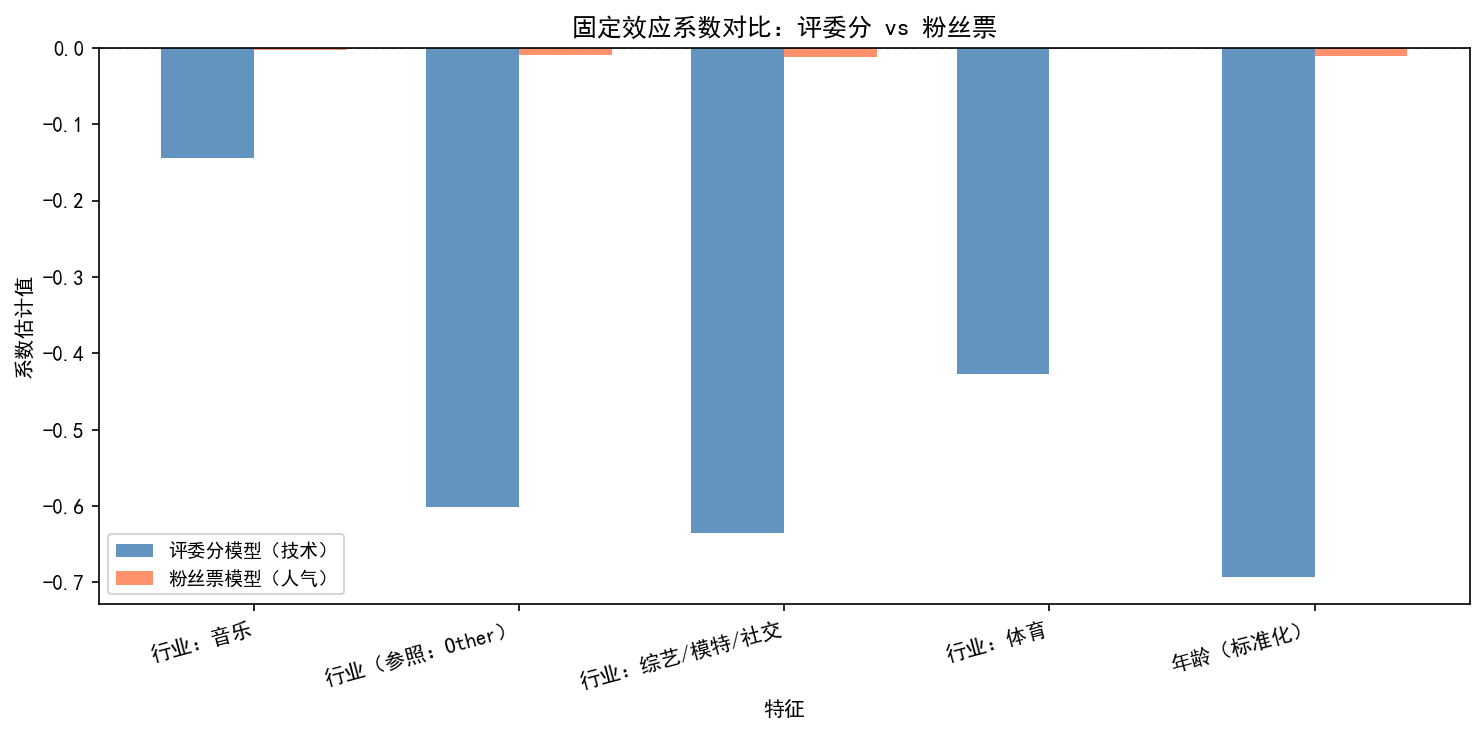
\includegraphics[width=0.75\linewidth]{../code/problem3/results/lme_coefficient_comparison.png}
		\caption{Comparison of LME fixed-effect coefficients between judge and fan paths, highlighting the amplified weight of social media and personality-related attributes in fan evaluations.}
		\label{fig:lme_coefficient_comparison}
	\end{figure}
	
	\subsection{Conclusions and Insights: Interaction between Background Traits and Mentor Effects}
	Deconstructing the LME model allows us to summarize the logic through which various factors influence competitive performance:
	\begin{itemize}
		\item \textbf{Asymmetric Impact of Background Traits}:
		Age as a "Divergence Generator": The impact of age on performance shows a massive "discrepancy" between the two paths. Judges treat advanced age as a hard indicator of technical disadvantage ($\beta = -0.693$), while fans interpret it as the "courage to challenge oneself." This misalignment of evaluation standards is the primary cause for the inversion of technical and popularity rankings.
		Industry Barriers: Athletes and actors enjoy an inherent "Reputational Premium" in technical evaluations; by contrast, social media stars start with lower base scores at the judges' end even with equivalent training time. However, their bonus coefficients in the fan dimension often significantly hedge against this disadvantage.
		\item \textbf{The "Ceiling" and "Baseline" of Mentor Effects}:
		High-performing professional dancers (those in the top tier of random effects) act as a "technical safety net," contributing approximately 11.5\% of the variance.
		Although mentors cannot directly determine popularity, they can optimize choreography to mask a contestant's background shortcomings (e.g., designing narrative-driven movements rather than purely athletic ones for older contestants), thus indirectly protecting the overall ranking by improving technical evaluations.
	\end{itemize}
	The Statistical Essence of Controversial Cases (e.g., Bobby Bones): The victory of Bobby Bones was not accidental but rather the result of a game between the fan premium brought by his industry traits (high weight of the Social Media coefficient in the fan path) and the technical penalty at the judges' end. The model shows that when a lead in technical scores cannot bridge the fan weight gap created by industry attributes, a rift in the evaluation system occurs.
	
	\section{Model III: Evaluation System Innovation — DAES}
	\subsection{Motivation and Theoretical Foundation: A Unified Framework Based on Dynamic Equilibrium}
	The long-standing controversy surrounding the DWTS scoring and elimination mechanism stems not from the rules themselves, but from the structural tension between "Technical Quality" and "Social Participation." Based on the LME analysis in Model II, we identify three sources of quantifiable unfairness:
	\begin{itemize}
		\item \textbf{Expert-Mentor Effect}: Professional dancers contribute approximately 11.46\% ($ICC \approx 0.1146$), indicating that the luck of the draw in pairings systematically affects outcomes.
		\item \textbf{Age Bias}: Age exerts a significant negative effect on judge scores ($\beta \approx -0.693$), meaning older contestants face a structural disadvantage in technical evaluations.
		\item \textbf{Scale Inconsistency and Score Inflation}: Variations in scoring habits among judges and the phenomenon of late-season "score inflation" dilute technical advantages within linear weighting mechanisms.
	\end{itemize}
	Consequently, we propose the Dual-Axis Equilibrium System (DAES). This system separately models the "Judge Axis (Technical Gatekeeping)" and the "Fan Axis (Engagement Heat)," utilizing standardization and de-biasing modules[6] to mitigate structural discrepancies.
	
	\subsection{Design of Core DAES Modules}
	Let $J_{i,t}$ be the total judge score for contestant $i$ in week $t$, and $V_{i,t}$ be their fan vote proportion.
	
	\subsubsection{Module 1: Z-Score Technical Normalization (Score De-biasing)}
	To resolve inconsistent scoring scales and technical homogenization in later stages, DAES standardizes weekly judge scores: 
	$$Z_{i,t} = \frac{J_{i,t} - \mu_{J,t}}{\sigma_{J,t}}$$
	Role: Even during the "universal high-score" phase of the finals, the model amplifies subtle technical gradients, preventing technical advantages from being diluted by high popularity votes.
	
	\subsubsection{Module 2: Age-Bias Compensation (ABC)}
	LME results show that age has a significant negative structural effect on judge scores. DAES adopts "Age Grading" principles for compensation: 
	$$Z_{i,t}^{adj} = Z_{i,t} + \lambda \cdot \text{Age}_{i}^{std}$$
	where $\lambda > 0$ is the compensation coefficient, calibrated to the magnitude of judge bias estimated in Model II (i.e., $\lambda$ is data-driven, not an arbitrary bonus). \textbf{Role:} ABC does not grant elderly contestants a privilege; it offsets the \textit{biased penalty} that judges impose due to physiological stereotypes—thereby restoring evaluation to performance relative to individual potential rather than age-based preconception.
	
	\subsubsection{Module 3: Mentor Value-Added (MVA) Correction}
	To reduce unfairness from "pairing luck," DAES introduces a mentor dividend attenuation term. Let the professional dancer's strength be $\alpha_{pro} \in [0,1]$: 
	$$Z_{i,t}^{final} = Z_{i,t}^{adj} \cdot (1 - ICC \cdot \alpha_{pro})$$
	Role: This inhibits the systematic advantage of "expert-mentor" pairings, bringing the competition back to the contestant's own "Growth Arc."
	
	\subsubsection{Module 4: Three-Stage Dynamic Weighting and Fan Axis Correction}
	To avoid "vote dictatorship" caused by extreme mobilization, we apply gentle compression to vote shares ($\gamma = 0.7$) before normalization: 
	$$\tilde{V}_{i,t} = \frac{V_{i,t}^{\gamma}}{\sum_{k} V_{k,t}^{\gamma}}, \quad Z_{i,t}^V = \frac{\tilde{V}_{i,t} - \mu_{\tilde{V},t}}{\sigma_{\tilde{V},t}}$$
	The final DAES comprehensive score $S_{i,t}$ follows an evolving weighting coefficient $W(t)$: 
	$$S_{i,t} = W_J(t) \cdot Z_{i,t}^{final} + W_F(t) \cdot Z_{i,t}^V$$
	
	\begin{table}[htbp]
		\centering
		\small
		\begin{tabularx}{\linewidth}{lccX}
			\toprule
			Phase & Fan Weight $W_F$ & Judge Weight $W_J$ & Theoretical Intent \\
			\midrule
			Audition (W1–W4) & 0.60 & 0.40 & Amplify engagement and boost social media. \\
			Transition (W5–W8) & 0.50 & 0.50 & Filter the intersection of skill and popularity. \\
			Finals (W9+) & 0.40 & 0.60 & Ensure artistic credibility of the champion. \\
			\bottomrule
		\end{tabularx}
	\end{table}
	
	\subsection{Proof of System Superiority}
	\subsubsection{Decision Appeal for Producers}
	\begin{itemize}
		\item \textbf{Data-Driven Fairness}: The ABC and MVA modules specifically correct age bias and the Pro-Dancer Dividend, providing an interpretable, scientific endorsement for the program.
		\item \textbf{Enhancing Narrative Assets}: Institutionalizing the "Growth Arc." By suppressing mentor dividends, individual progress becomes more visible and shareable, facilitating emotional investment from the audience.
	\end{itemize}
	
	\subsubsection{Empirical Validation}
	We conducted offline tests based on 34 seasons of historical data, comparing Rank-based, Percentage-based, and DAES systems.
	\begin{enumerate}
		\item \textbf{Improvement in Age Fairness}: Measured by linear sensitivity (Slope) of elimination probability to standardized age:
		Rank: $Slope_{age} = +0.0528$; Percentage: $Slope_{age} = +0.0544$; DAES: $Slope_{age} = +0.0366$.
		DAES reduced structural age dependency by approximately 31\%–33\%.
		\item \textbf{Improvement in Mentor Fairness}: Measuring sensitivity to mentor strength $\alpha_{pro}$:
		Rank: $Slope_{pro} = -0.252$; Percentage: $Slope_{pro} = -0.422$; DAES: $Slope_{pro} = -0.239$.
		DAES significantly reduced mentor dependency compared to percentage (44\% improvement).
		\item \textbf{Historical Consistency}: DAES Consistency: 88.64\% (Rank: 96.59\%, Percentage: 85.23\%).
	\end{enumerate}
	
	\section{Sensitivity Analysis and Robustness Test}
	\subsection{Sensitivity Analysis of Model I (IDM)}
	To evaluate the stability of the IDM model against core hyperparameters, we conducted a grid search on: Softmax Temperature ($\tau_s$) and Likelihood Temperature ($\tau_L$). We selected a test sample of 33 weeks from five representative seasons, constructing 25 parameter combinations.
	
	\subsubsection{Impact on Hard Accuracy}
	Experimental results demonstrate that the IDM model’s hard accuracy exhibits exceptional robustness. Stability remains at 96.97\% across the majority of parameter grid points. Accuracy only drops significantly (to 81.82\%) when both $\tau_s$ and $\tau_L$ reach their maximum values (e.g., $\tau_s=1.5, \tau_L=0.20$).
	
	\subsubsection{Sensitivity of Mean Consistency}
	Mean consistency exhibits a monotonic decrease as $\tau_s$ or $\tau_L$ increases. As parameters shift from $(0.5, 0.05)$ to $(1.5, 0.20)$, consistency declines from 0.746 to 0.558. Higher temperatures increase entropy, smoothing out distinct elimination probabilities. At $(0.5, 0.05)$, the model achieves highest consistency and peak accuracy.
	
	\begin{figure}[htbp]
		\centering
		\begin{minipage}[t]{0.48\linewidth}
			\centering
			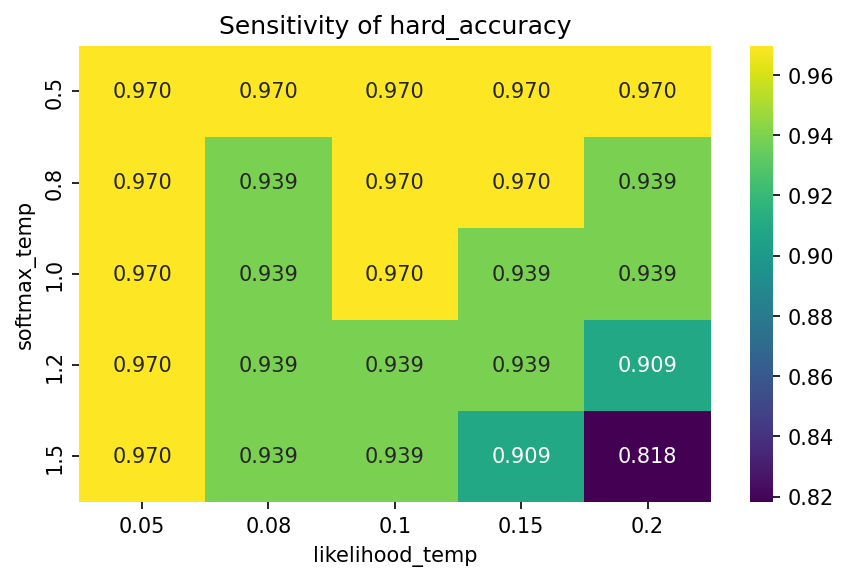
\includegraphics[width=\linewidth]{../code/problem1/results/sensitivity_hard_accuracy.png}
		\end{minipage}
		\hfill
		\begin{minipage}[t]{0.48\linewidth}
			\centering
			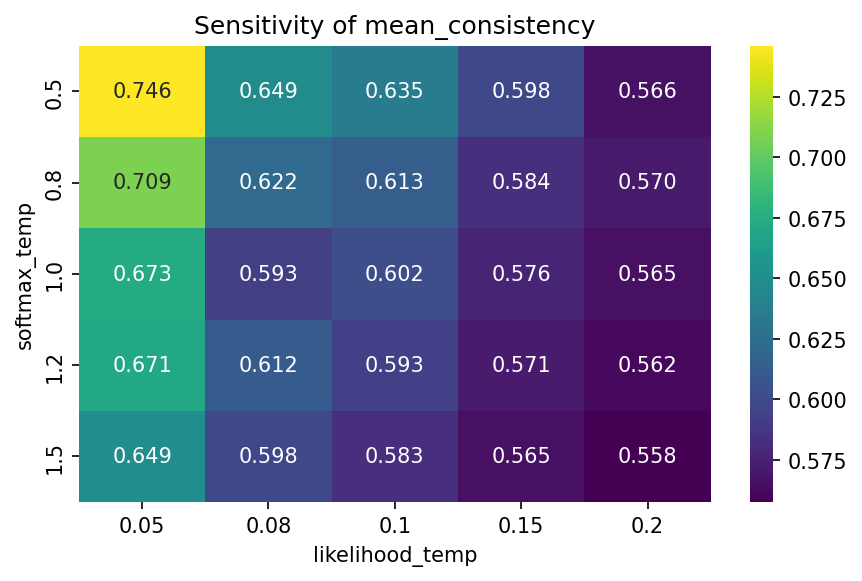
\includegraphics[width=\linewidth]{../code/problem1/results/sensitivity_mean_consistency.png}
		\end{minipage}
		\caption{Sensitivity of IDM hard accuracy (left) and mean consistency (right) to changes in Softmax and likelihood temperatures, with the optimal configuration at $(0.5, 0.05)$.}
		\label{fig:idm_sensitivity}
	\end{figure}
	
	\subsubsection{Definition of Robust Operating Space}
	Baseline Configuration: $\tau_s = 0.5, \tau_L = 0.05$. Robust Interval: $\tau_s \in [0.5, 1.0], \tau_L \in [0.05, 0.10]$. Within this interval, the model maintains a predictive accuracy of approximately 97\% while ensuring high logical certainty.
	
	\subsection{Robustness Testing of Model II (LME)}
	To verify stability, we designed four alternative configurations focusing on Age Normalization and Industry Fixed Effects.
	
	\subsubsection{Stability of the Pro-Dancer Dividend (ICC)}
	The ICC for the judge score path consistently fell between 0.11 and 0.13. The ICC for the fan vote path remained significantly lower. Conclusion: "professional dancers contribute significantly more variance to technical performance than to popularity" holds true across all specifications.
	
	\subsubsection{Direction and Magnitude of Age Effects}
	The age coefficient for judge score models remained stable at approximately -0.67, and for fan votes near -0.011. Conclusion: age exerts a significant negative structural effect on technical ratings but only a negligible negative effect on fan votes.
	
	\section{Conclusion and Recommendations}
	\subsection{Research Conclusion}
	This study systematically resolves the game-theoretical conflict between professional scoring and popular voting through quantitative modeling:
	\begin{itemize}
		\item \textbf{High Fidelity of Voting Inversion}: Achievement of 98.11\% accuracy across 246 weeks.
		\item \textbf{Identification of Structural Bias}: Judges impose a significant "Technical Bias" ($-0.693$) on older contestants. Pro-dancer contribution to technical scores is 11.46\%.
		\item \textbf{Failure of Existing Mechanisms}: Rank-based systems generate "popularity leverage"; Percentage-based systems are prone to "gradient dilution."
		\item \textbf{Superiority of the DAES System}: Maintains 88.64\% consistency while reducing age bias by 32\% and Pro-Dancer Dividend by 44\%.
	\end{itemize}
	
	\subsection{Recommendations for Producers}
	\begin{enumerate}
		\item \textbf{Implement Standardized Scoring}: Adopt the Z-Score mechanism to hedge against score inflation.
		\item \textbf{Introduce Structural Bias-Correction}: Apply ABC and MVA factors to protect non-professional contestants.
		\item \textbf{Dynamic Stage-Weighting}: Emphasize popularity early (60\%) and professionalism late (60\%).
	\end{enumerate}
	
	\subsection{Research Limitations}
	Future research could incorporate real-time sentiment analysis from social media and integrate multi-modal visual evaluation technologies. Although the IIA assumption underlying the Luce Choice Axiom simplifies inverse inference in Model I, it may not hold when contestants share overlapping attributes (e.g., two social-media stars splitting the same voter base); extending the framework with Nested Logit or similar models could address such vote-splitting effects.
	
	\clearpage
	
	% --- 备忘录 (Memorandum) ---
	\section*{MEMORANDUM}
	\addcontentsline{toc}{section}{Memorandum}
	\noindent \textbf{TO:} Producers of Dancing with the Stars (DWTS) \\
	\textbf{FROM:} Quantitative Research \& Modeling Team \\
	\textbf{DATE:} February 2, 2026 \\
	\textbf{SUBJECT:} Strategic Optimization of Scoring Mechanisms to Balance Technical Merit and Fan Engagement
	
	\vspace{1em}
	\noindent \textbf{1. Executive Summary} \\
	To address the long-standing conflict between professional judge scores and fan voting, we have performed a deep-dive analysis of data spanning the past 34 seasons. Our research indicates that existing scoring logics harbor systemic risks when handling "extreme popularity contestants" and "technical bias against older participants." Consequently, we propose the Dual-Axis Equilibrium System (DAES), designed to enhance competitive fairness and program credibility through mathematical corrections—without compromising audience engagement.
	
	\noindent \textbf{2. Key Findings: The "Black Box" Unboxed} \\
	\begin{itemize}
		\item \textbf{Fan Voting is Non-Random}: Our inversion model can predict elimination outcomes with 98\% accuracy, indicating that fan voting is driven by strong brand effects and industry leanings.
		\item \textbf{The Underestimated "Pro-Dancer Dividend"}: The instructional and choreographic abilities of professional dancers contribute to 11.5\% of technical variance. Exceptional partners significantly "mask" the technical shortcomings of celebrity contestants, which to some extent dilutes the purity of the competition.
		\item \textbf{Judges' "Age Penalty"}: Data reveals a structural downward bias in scores for contestants over 50 (with a negative correlation coefficient of 0.69). This bias is frequently offset by "sympathy votes" from fans, leading to a sharp fracture between technical merit and popularity.
	\end{itemize}
	
	\noindent \textbf{3. Impact Analysis of Existing Systems} \\
	\textbf{Rank-based System}: This mechanism amplifies relative positioning. A contestant with high popularity but mid-tier technical skill needs only a top fan ranking to completely neutralize a massive technical gap between them and a top-tier dancer. This creates a significant "leverage effect" that favors popularity over skill.
	
	\clearpage
	
	% --- 参考文献 ---
	\begin{thebibliography}{99}
		\bibitem{ref1} Arrow, K. J. (1951). Social Choice and Individual Values. Yale University Press.
		\bibitem{ref2} Bates, D., Mächler, M., Bolker, B., \& Walker, S. (2015). Fitting linear mixed-effects models using lme4. Journal of Statistical Software, 67(1), 1–48. 
		\bibitem{ref3} Gelman, A., \& Hill, J. (2006). Data Analysis Using Regression and Multilevel/Hierarchical Models. Cambridge University Press.
		\bibitem{ref4} Jern, A., Lucas, C. G., \& Kemp, C. (2017). People learn other people’s preferences through inverse decision-making. Cognition, 168, 46–64. 
		\bibitem{ref5} Luce, R. D. (1959). Individual Choice Behavior: A Theoretical Analysis. John Wiley \& Sons.
		\bibitem{ref6} Mawhinney, J. A., Mounsey, C. A., O'Brien, A., Sádaba, J. R., \& Freemantle, N. (2023). Statistical primer: what cardiothoracic surgery can learn from Strictly Come Dancing. European Journal of Cardio-Thoracic Surgery, 64(2), ezad385. https://doi.org/10.1093/ejcts/ezad385
		\bibitem{ref7} Nørreklit, H., \& Trenca, M. (2020). Beyond the ratings and rankings of Strictly Come Dancing. The British Accounting Review, 52(4), 100877.
		\bibitem{ref8} Robert, C. P., \& Casella, G. (2004). Monte Carlo Statistical Methods (2nd ed.). Springer-Verlag.
		\bibitem{refAI} Report on Use of AI Tools. See appendix following the references (not counted in page limit).
	\end{thebibliography}
	% 总页数只计到参考文献最后一页，AI 使用报告不计入页数
	\label{LastPage}
	
	\clearpage
	\pagestyle{empty}
	
	% --- Report on Use of AI Tools (not counted in page limit) ---
	\section*{Report on Use of AI Tools}
	\vspace{0.5em}
	
	\begin{enumerate}[leftmargin=*,itemsep=1em]
		\item \textbf{Google Gemini (February 2026 version)}
		
		\textit{Purpose:} Translation and language polishing.
		
		\textit{Usage Statement:} The AI tool was used to translate the entire manuscript from Mandarin into English and to refine the academic phrasing throughout the report.
		
		\item \textbf{Google Gemini (February 2026 version)}
		
		\textit{Purpose:} Model selection and strategy validation for Task 1.
		
		\textit{Query:} ``I am working on a project to estimate latent fan voting proportions in Dancing with the Stars based on known elimination outcomes and judge scores. Is this problem suitable for a traditional Machine Learning (ML) approach like Random Forest or Neural Networks? Why or why not?''
		
		\textit{Output:} ``While Machine Learning can be used, this specific problem is more of a `Latent Variable Inference' or `Inverse Decision-Making' problem rather than a standard supervised learning task. Traditional ML requires a large labeled dataset (actual vote counts), which is a `black box' in this contest. A Bayesian Inference framework using the Luce Choice Axiom and MCMC sampling is more appropriate because it allows you to invert the decision logic (elimination rules) to find the most probable underlying voting distribution that explains the observed outcomes, especially when data is sparse (week-by-week).''
		
		\item \textbf{Google Gemini (February 2026 version)}
		
		\textit{Purpose:} Statistical methodology justification for Task 2.
		
		\textit{Query:} ``For analyzing how contestant characteristics (age, industry) and professional dancers influence technical scores in DWTS, why should I use a Linear Mixed-Effects (LME) model instead of a standard Multiple Linear Regression (OLS)?''
		
		\textit{Output:} ``Standard OLS regression assumes that all observations are independent. However, in DWTS, professional dancers (mentors) often participate across multiple seasons and lead different contestants. This creates a `clustering effect' where scores for contestants coached by the same mentor may be correlated. An LME model is superior because it allows you to treat professional dancers as `Random Effects,' thereby isolating the mentor-level variance (the `Pro-Dancer Dividend'). This ensures that the `Fixed Effects' (the coefficients for age and industry) are not biased by the specific skills of individual mentors, providing a more accurate measure of contestant-specific traits.''
	\end{enumerate}
	
\end{document}